\chapter{实验内容}
本章介绍本工作的实验方案、实验装置及测量过程，并说明与后续数据分析密切相关的关键实验条件与参数。
\section{实验方案}
基于先前极具参考价值的$^{16}\mathrm{O}$+$^{152,150,148,144}\mathrm{Sm}$ 体系的工作\cite{talon1981coulomb}，本工作也选取形变核 $^{152}\mathrm{Sm}$ 为靶核，其四极和八极形变参数分别为 $\beta_2 = 0.308$、$\beta_4 = 0.127$，基态为$0^+$态，第一、二激发态（$2^+$ 和 $4^+$）的激发能分别为 121~keV 和 366~keV\cite{nudat}。与 $^{154}\mathrm{Sm}$ 第一激发态的激发能（82~keV）相比，$^{152}\mathrm{Sm}$ 的激发能更高，既属于易于激发的大形变核，又避免因激发能过小对探测器分辨能力提出过高要求。为了避免完全重复的测量，本工作选用与先前工作相似的$^{18}\mathrm{O}$作为弹核。
相较于已有工作，本实验力求在以下几个方面取得改进：
% 1. 对能量有更高的分辨，更清晰地区分开基态和2+态的情况。
% 2. 在更宽的能量范围42（0.7VB）-90（1.5VB ）MeV，以更小的能量间隔、角度间隔测量体系的弹性散射角分布，给出更细致的光学势信息。
% 3. 最终从角分布中提取出光学势，并由此调查阈异常在大形变核中的情况。
（1）提高能量分辨率，实现基态与第一激发态散射峰的可靠区分；

（2）在更宽能区内42（0.7VB）-90（1.5VB ）MeV，以更密集的能点和角度步长测量角分布；

（3）系统提取光学势参数，研究其能量依赖行为及阈异常特征。

完成实验目标的主要难点在于，经过理论计算，实验中的动量分辨需要达到 0.06\% 的水平才能区分弹性散射反应道和准弹性散射反应道的粒子。因此本次实验需要在中国原子能科学研究院的 HI-13 串列加速器 Q3D 磁谱仪终端上开展，该磁谱仪配合位置探测器的探测体系拥有0.01\%级别的分辨潜力。

在获得了弹性散射角分布以及准弹性散射角分布数据后，就可以使用光学模型对数据进行拟合，得到各个能量下的光学势参数，从而调查光学势的能量相依性以及色散关系。
\section{实验设置}
\subsection{束流线}
本实验在中国原子能科学研究院的 HI-13 串列加速器 Q3D 磁谱仪终端上开展。
实验设施整体情况如图\ref{装置}。
\begin{figure}[h]
\centering
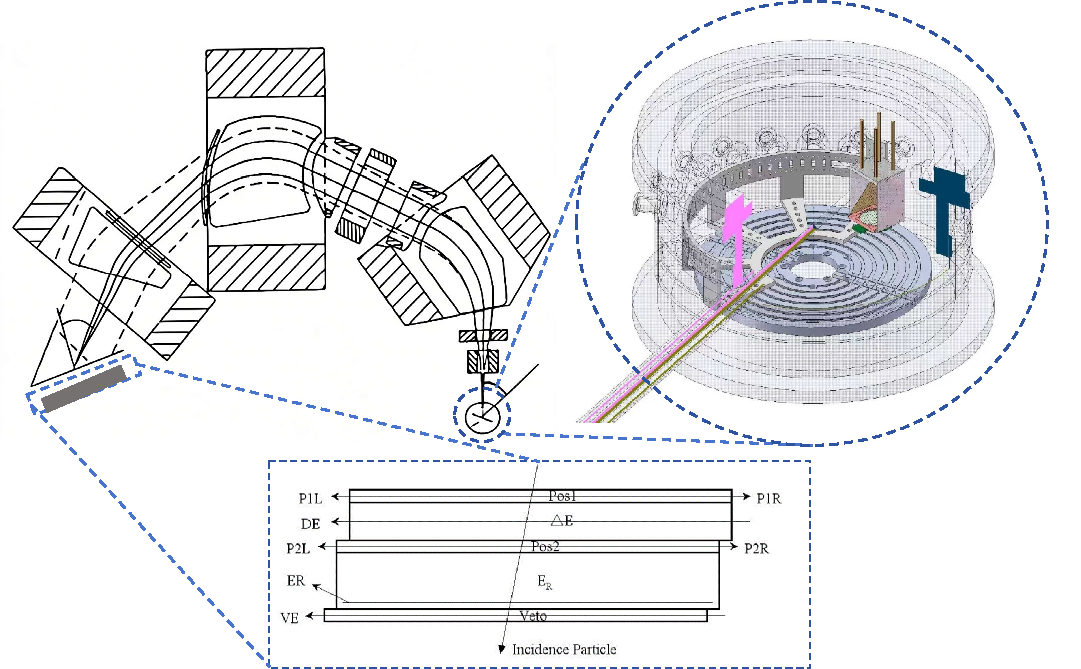
\includegraphics[width=0.95\linewidth]{images/装置.pdf}
\caption{实验设施示意图}
\label{装置}
\small 左上方为Q3D磁谱仪示意图，右上方为反应靶室示意图，下方为焦面探测器示意图。
\end{figure}

使用$^{18}\mathrm{O}$ 束流（流强约20~$e$nA）轰击厚度约 10~$\mathrm{\mu} \mathrm{g/cm^2}$ 的$^{152}\mathrm{Sm}$ 靶（碳底衬厚度约  10~$\mathrm{\mu} \mathrm{g/cm^2}$），能量分别为 72、68、64、60、56 和52~MeV（相应于0.79$V_\mathrm{B}$～1.09$V_\mathrm{B}$，$V_\mathrm{B} \approx 66$~MeV\cite{wen2022new}）。在反应靶室中从25°-160°水平放置28块硅PIN探测器用于测量准弹性角分布；在25°放置3块硅PIN探测器用于束流监视器，测量卢瑟福散射。束流在反应靶室轰击靶后可以进入Q3D磁谱仪，经过磁谱仪偏转后进入焦面靶室。在焦面靶室放置一块五层的焦面探测器用于测量弹性散射角分布，其有效探测长度为50~cm，充入80~torr的CF4气体，并为每一层的一端加上了1000~V的高压。Q3D磁谱仪可以在-20～140°的范围进行旋转。
\subsection{探测体系}
\subsubsection{PIN阵列}
如图\ref{装置}中的反应靶室所示，31块厚度为300~$\mu$m 的硅PIN探测器被规律地安装在靶室支架的孔后。这些PIN探测器都采用混合三α标准源进行能量刻度与分辨测试。，能谱如图\ref{PIN测试}所示，可以清晰辨认出各个α源的峰，能量分辨普遍在1\%的水平。
\begin{figure}[h]
\centering
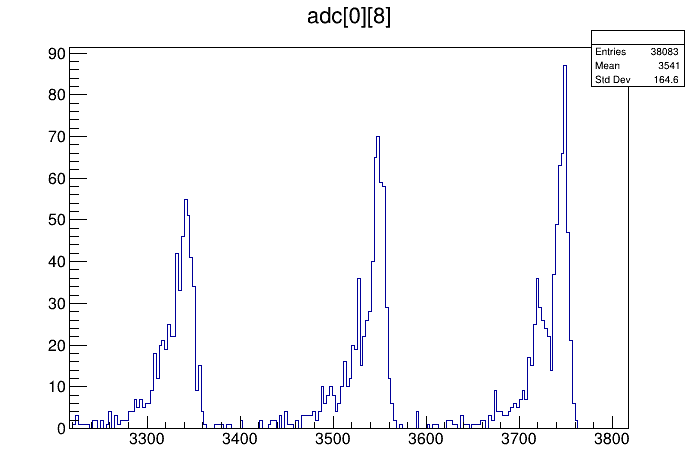
\includegraphics[width=0.95\linewidth]{images/PIN测试.png}
\caption{PIN探测器测试能谱图}
\label{PIN测试}
\end{figure}

\subsubsection{焦面探测器}
焦面探测器是一个五层的气体电离室，其有效探测长度（窗口）为50 cm，通过粒子在各层的能损来还原入射位置等信息，结构如图\ref{焦面探测器结构}所示。探测器使用4 μm厚的透明Mylar膜作为窗膜，各层之间以厚度为1 μm的镀铝Mylar膜分隔。内部充入常温下100 torr的CF₄气体。

第一层和第三层均为位置探测器，厚度为1 cm，每层中间都设有一根从两端引出的电阻丝。实际测得第一层阳极丝的电阻值为13.67～13.76 kΩ，第三层为14.58～14.75 kΩ。加高压时，第一层在1000 V下漏流为0；第三层在1000 V下漏流为0.02 μA，最高可加至1100 V，此时漏流为0.025 μA。当粒子入射到这两层中，我们通过采集电阻丝两端的信号，利用电荷分除法得到入射的相对位置，并进一步结合第一层与第三层的位置信息重建粒子的径迹。理论上，这两层的位置分辨可达1 mm，但实际测试中第一层约为1.4 mm，第三层约为3 mm。

第二层为dE探测器，厚度同样为1 cm，中间设有一根仅从一端引出的镀金钨丝。其阳极丝电阻值为102～104 kΩ，加高压1300 V时漏流为0。该层较薄，用于获取粒子的能损信息，从而实现粒子鉴别等功能。由于第二层的能量分辨率约为6.5\%，单独使用时精度有限，因此实际实验中我们搭配时间计数器测量飞行时间，以获得更精确的粒子识别结果。

第四层为ER总能量探测器，第五层为Veto探测器。这两层在本实验中并未实际启用，故不再赘述。


\begin{figure}[h]
\centering
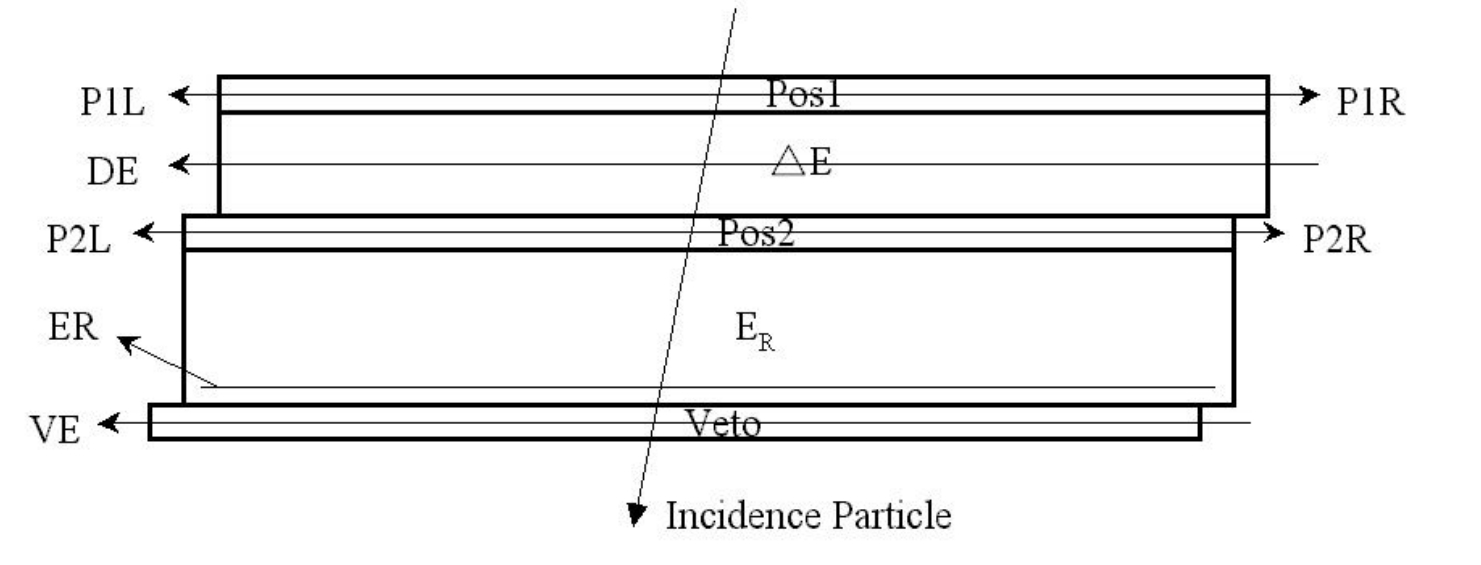
\includegraphics[width=0.95\linewidth]{images/焦面探测器.jpg}
\caption{焦面探测器探测器结构示意图}
\label{焦面探测器结构}
\end{figure}

焦面探测器拉丝是一个复杂的流程，这里记录一个稳健可行的方案：
（1）拧螺丝拆开探测器。注意不要一次卸下，多转几圈。
（2）拆下固定层的螺丝，再拆开固定膜的螺丝。
（3）焊接头处，将原本的断丝取出，清理膜内的断丝。
（4）用铁丝从内往外捅，将剩余的锡清理干净。
（5）制作“铜丝-弹簧-铜丝”段，要比隐藏在管道内的部分更长。可以使用两根铜丝扭在一起，强度更高。
（6）将“铜丝-弹簧-铜丝”段的一头扭出一个小钩子，将丝挂在钩子上，旋转钩子多缠绕几圈，再用锡焊上。清理多出来的线头。
（7）将“铜丝-弹簧-铜丝”段带着丝放入孔中，调整到合适位置，将铜丝在出口折一下。
（8）把丝缓慢放出拉到探测器另一头，留出足够长度后剪断丝。
（9）找一根粗的铜线，同样扭出一个小勾子，确保可以塞入孔中。将丝挂在钩子上旋转缠绕，随后焊上。清理多出来的线头。
（10）将粗铜线塞入孔中。小心调节粗铜线的位置，感受拉力，让线绷紧。随后也把粗铜线扭一下挂上孔固定。
（11）将两端的孔洞焊起来，再把漏出的丝和通往外部的丝焊起来，要提前放热缩管。
（12）清理膜上的垃圾碎屑。
（13）重新拧上螺丝。


在测试中，焦面探测器显示了良好的位置分辨性能。将焦面探测器的大部分窗口封住，只留出三个矩形缺口，随后使用3α源进行测试的结果如图\ref{focalTest}。图中纵坐标为dE能损，横坐标为第一层给出的相对位置，可以看到谱中位置探测器可以清晰分开三个矩形缺口入射的粒子，分辨经计算在1.4mm左右，而dE探测器可以区分开源的不同组分，能量分辨在8\%左右，满足实验要求。
\begin{figure}[h]
\centering
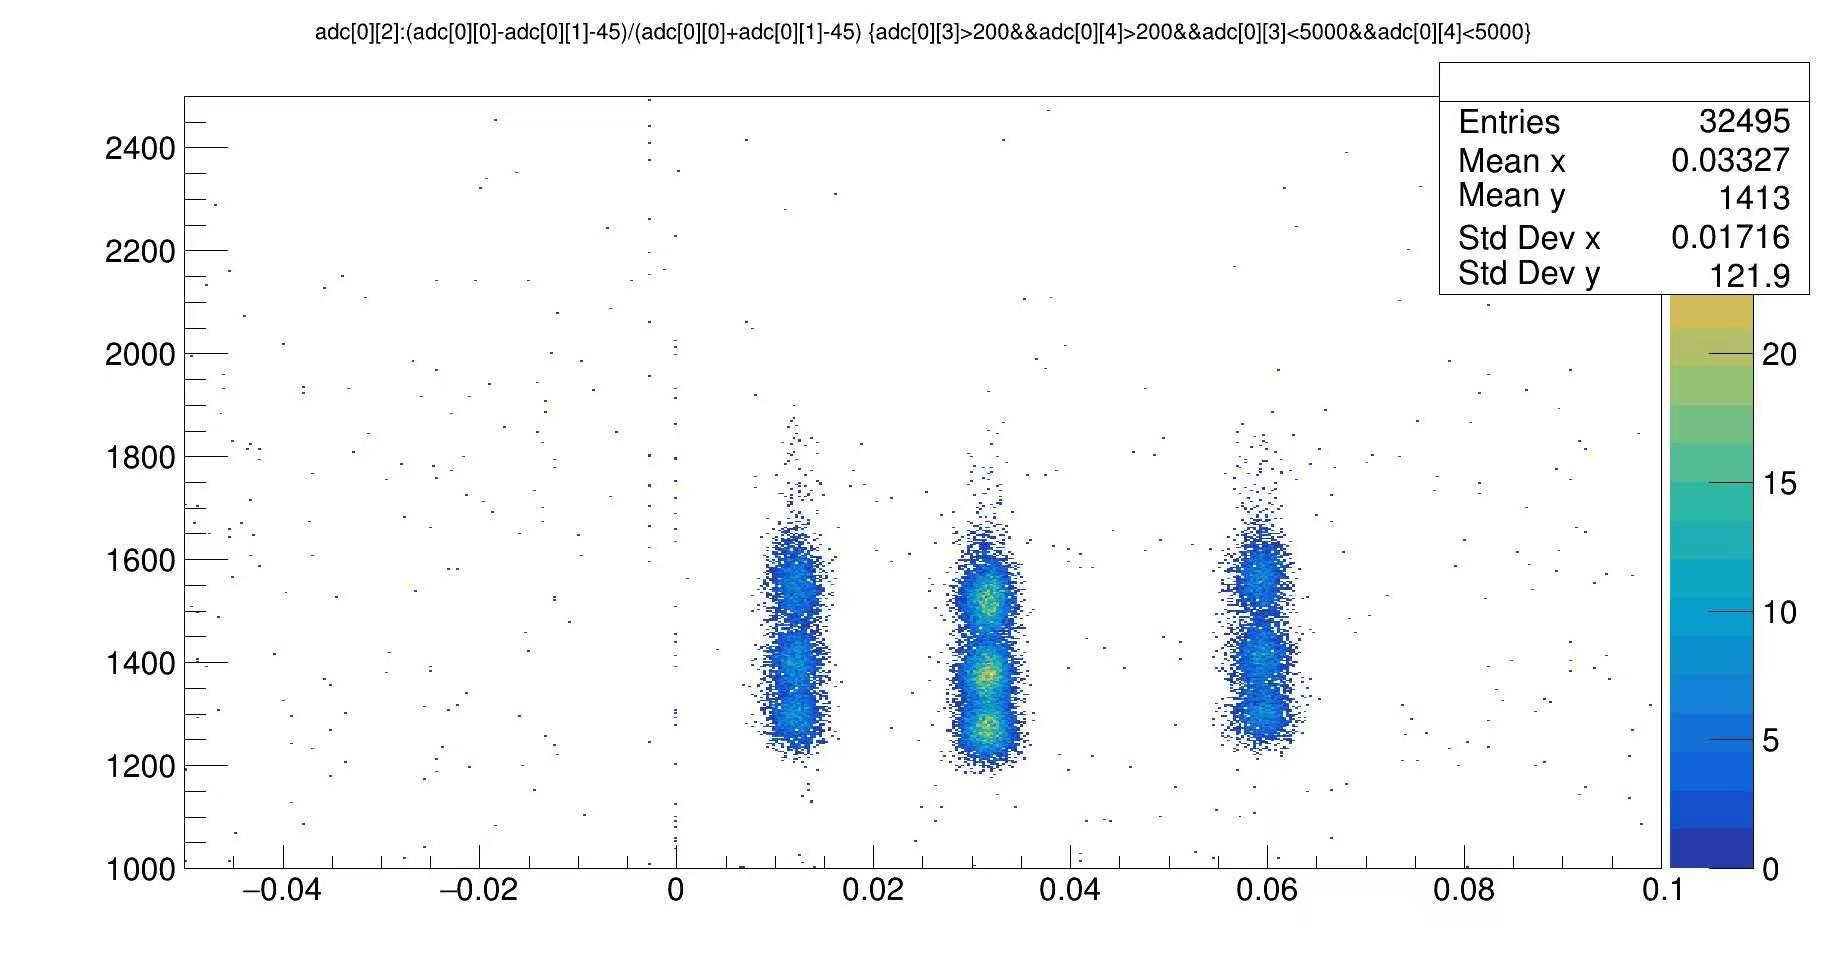
\includegraphics[width=0.95\linewidth]{images/focalTest.jpg}
\caption{焦面探测器探测器dE-位置谱}
\label{focalTest}
\end{figure}


%PSD探测器是Si材质的位置信息探测器。固定于一块板子上（我们称之为“小车”），该板子固定于一可移动轨道，可在大靶室腔体内左右两端自由移动，并在前后以及上下方向上小幅度移动。其中，小车左右移动时焦探保持静止，小车做上下前后运动时，焦探与小车相对静止。其位置控制按钮位于大靶室右侧，亦可在控制室右起第二个柜子上控制。

% 本次实验中用了两片一维PSD，PSD是一种硅材质的位置灵敏探测器。PSD由在平面硅衬底上的三层组成：P型层在表面，N型层在另一面，I层在它们中间。落在PSD上的入射光转换成光电子后由P型层上两端电极探测并形成光电流。而被电极收集到的光电流大小与光的入射点位置和电极之间的间距是成反比关系的。光电流大小与光的入射点位置和电极之间的间距成反比关系。

% 每片PSD共有6个引脚，其具体作用及接线在图\ref{小车}中已做说明。

% PSD的高压接在没有胶带的红色高压插件上的ch2上。（负压）
\subsection{电子学与获取系统}
本实验采用中国原子能科学研究院研制的 SPA02 型集成电荷灵敏前置放大器\cite{wang2020compact}作为前端读出电子学模块，用于 PIN 探测器及气体探测器信号的处理，其电路设计如图\ref{前放电路}。该前置放大器为16通道紧凑型结构，具有体积小、集成度高和多通道并行读出的特点，可方便地布置在探测器附近，从而缩短信号传输距离，减小外界电磁干扰及电缆引入噪声，提高信号保真度。
SPA02 的单通道核心采用电荷灵敏放大结构，主要由探测器偏置滤波网络、输入耦合电路以及反馈放大回路组成。探测器产生的电荷信号经积分转换后输出为幅度与入射粒子沉积能量成正比的电压脉冲，其反馈电阻和反馈电容参数可根据实验需求调节，以兼顾增益、动态范围及脉冲恢复时间。

前放Test信号如图\ref{前放Test}。性能测试表明，SPA02 系列前放具有较快的时间响应，典型脉冲上升时间约小于 6 ns，在低输入电容条件下等效噪声约为 1.5 keV，适合弱信号探测及高计数率实验环境。对于硅探测器系统，其能量分辨性能良好，能够满足核反应实验中对粒子能量测量的要求。

在本实验中，PIN 探测器输出信号幅度较小，对前端电子学噪声要求较高；气体探测器信号上升沿较缓、幅度变化范围较大，对放大器稳定性和动态范围也提出了要求。SPA02 前置放大器兼具低噪声、快响应和多通道集成等优点，可同时满足两类探测器的信号读出需求，为后续能谱分析、粒子鉴别及角分布测量提供可靠保障。



为了方便接线，PIN探测器使用了SPA02的16通道板，实物如图\ref{前放16}；而焦面探测器使用了基于SPA02核心的单通道前放，实物如图\ref{前放1}。将焦面探测器各层的引出与小前放相连后，可以进行加高压、输入Test信号等操作，并且可以将初步放大后的信号输出至MSCF主放。
而PIN探测器则连接到传统的原子能院自研SPA前放，然后同样输出至主放MSCF主放。主放则将放大后的信号输出到CAEN V785获取插件。获取插件都插在CAEN的VME获取机箱上，通过控制卡与电脑进行通信。


\begin{figure}[h]
\centering
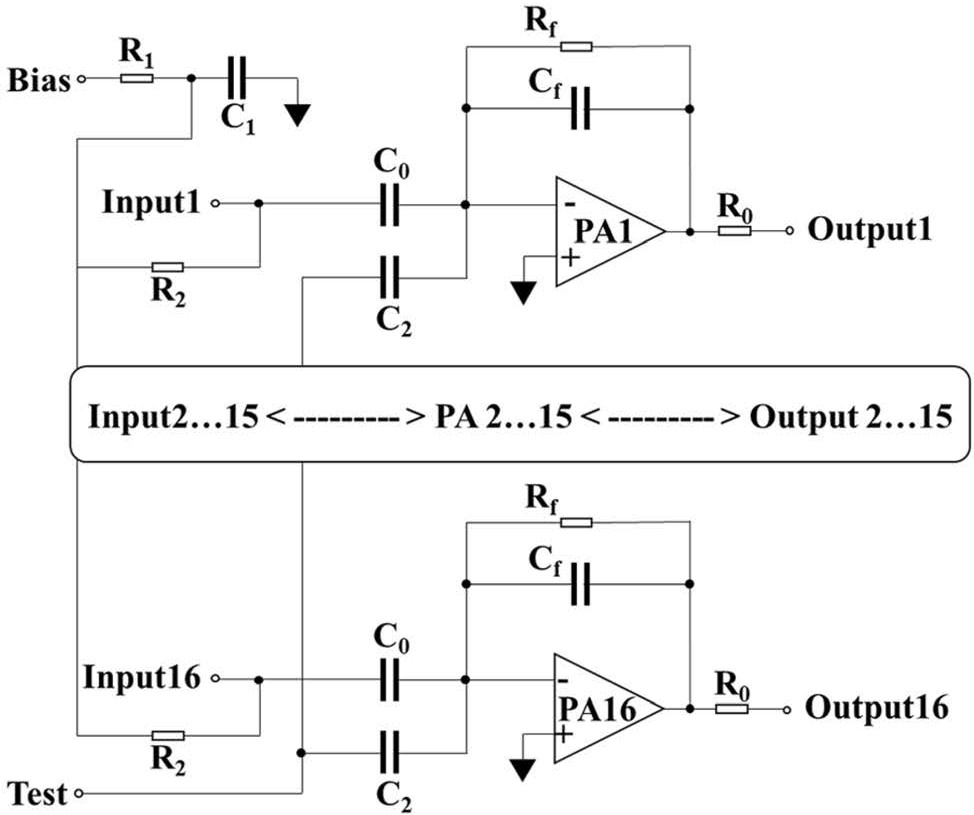
\includegraphics[width=0.5\linewidth]{images/前放电路.jpg}
\caption{前置放大器的电路设计图}
\label{前放电路}
\end{figure}


\begin{figure}[h]
\centering
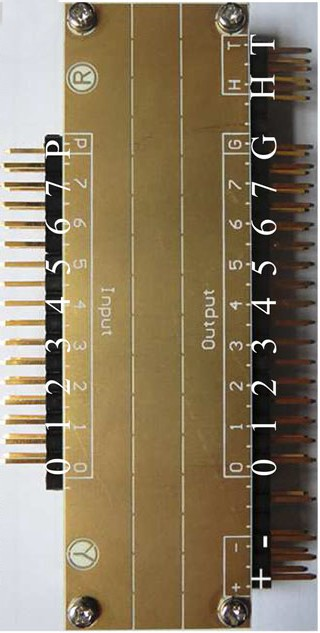
\includegraphics[width=0.32\linewidth]{images/前放16.jpg}
\caption{PIN探测器使用的前置放大器实物图}
\label{前放16}
\end{figure}

\begin{figure}[h]
\centering
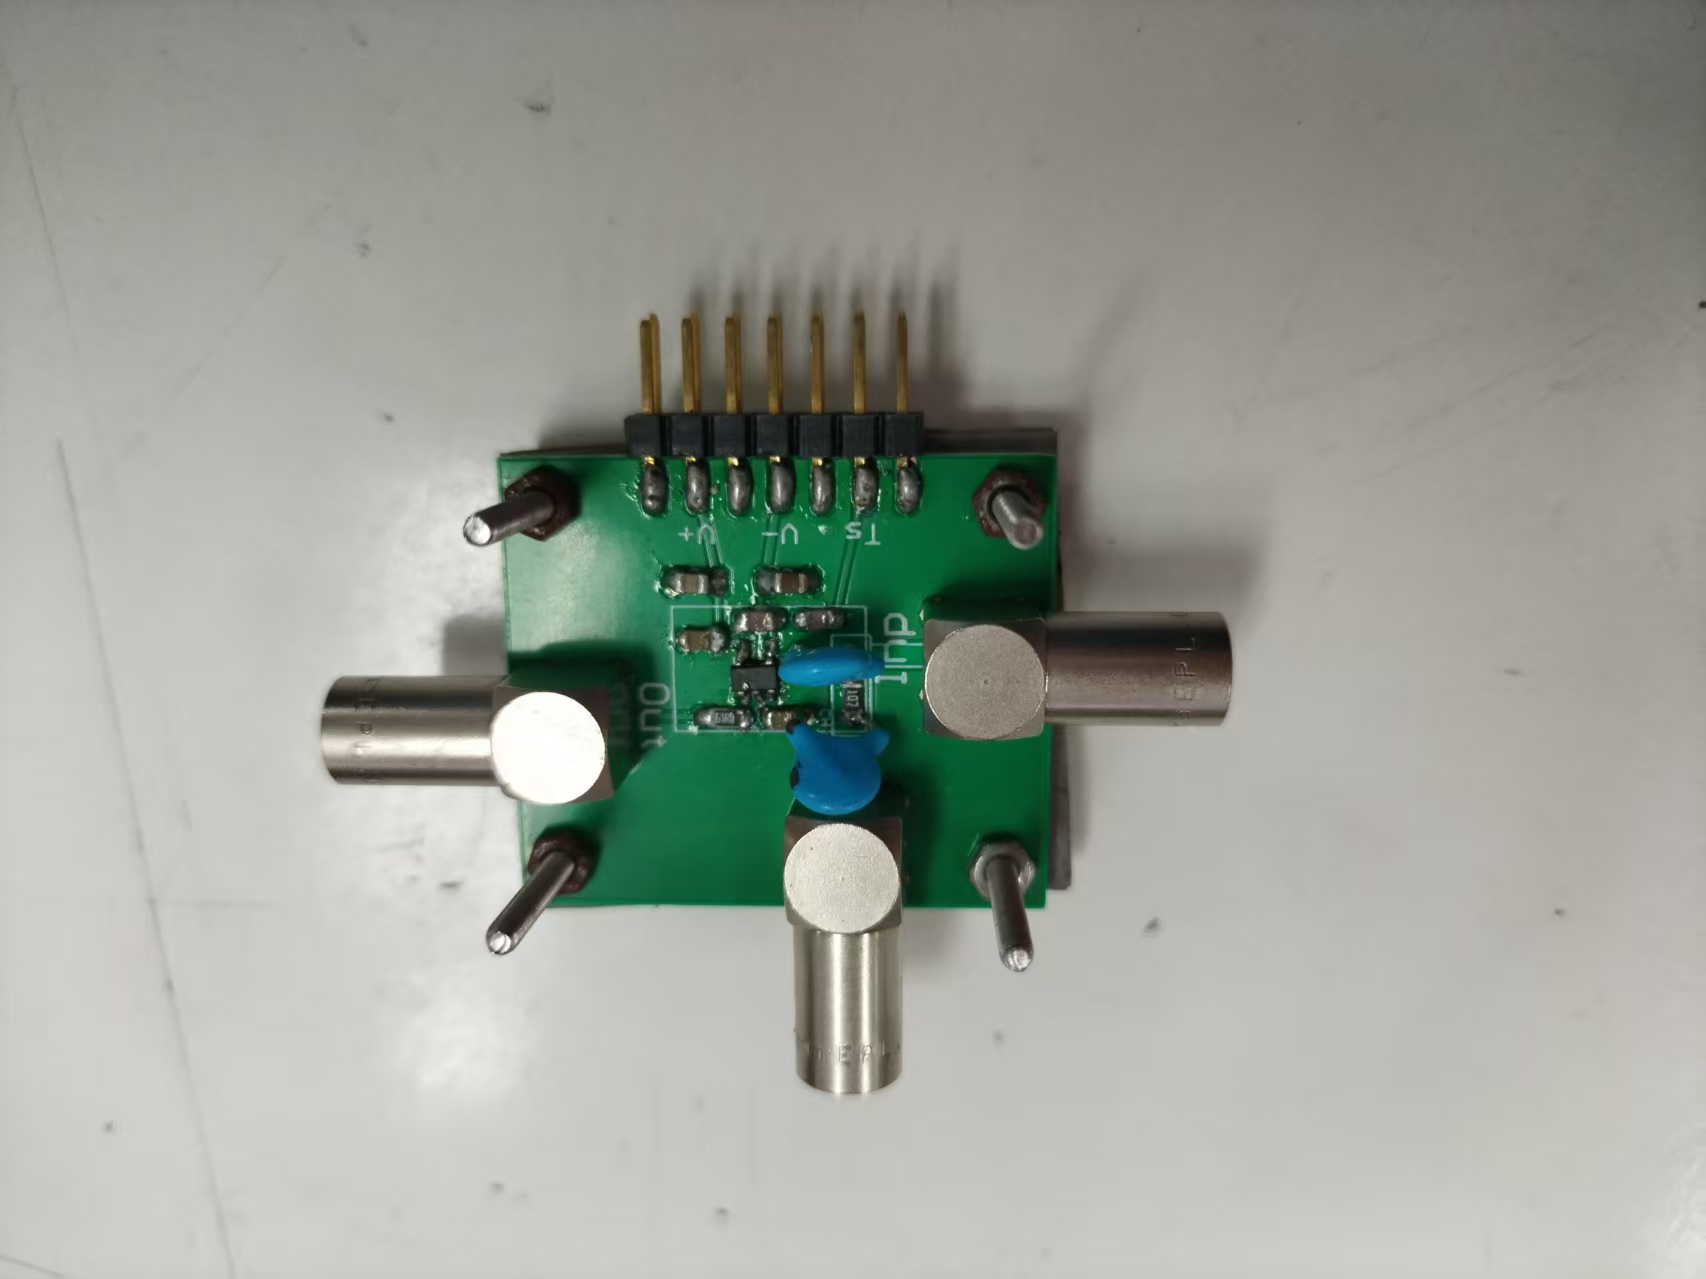
\includegraphics[width=0.6\linewidth]{images/前放.jpg}
\caption{焦面探测器使用的前置放大器实物图}
\label{前放1}
\end{figure}

\begin{figure}[h]
\centering
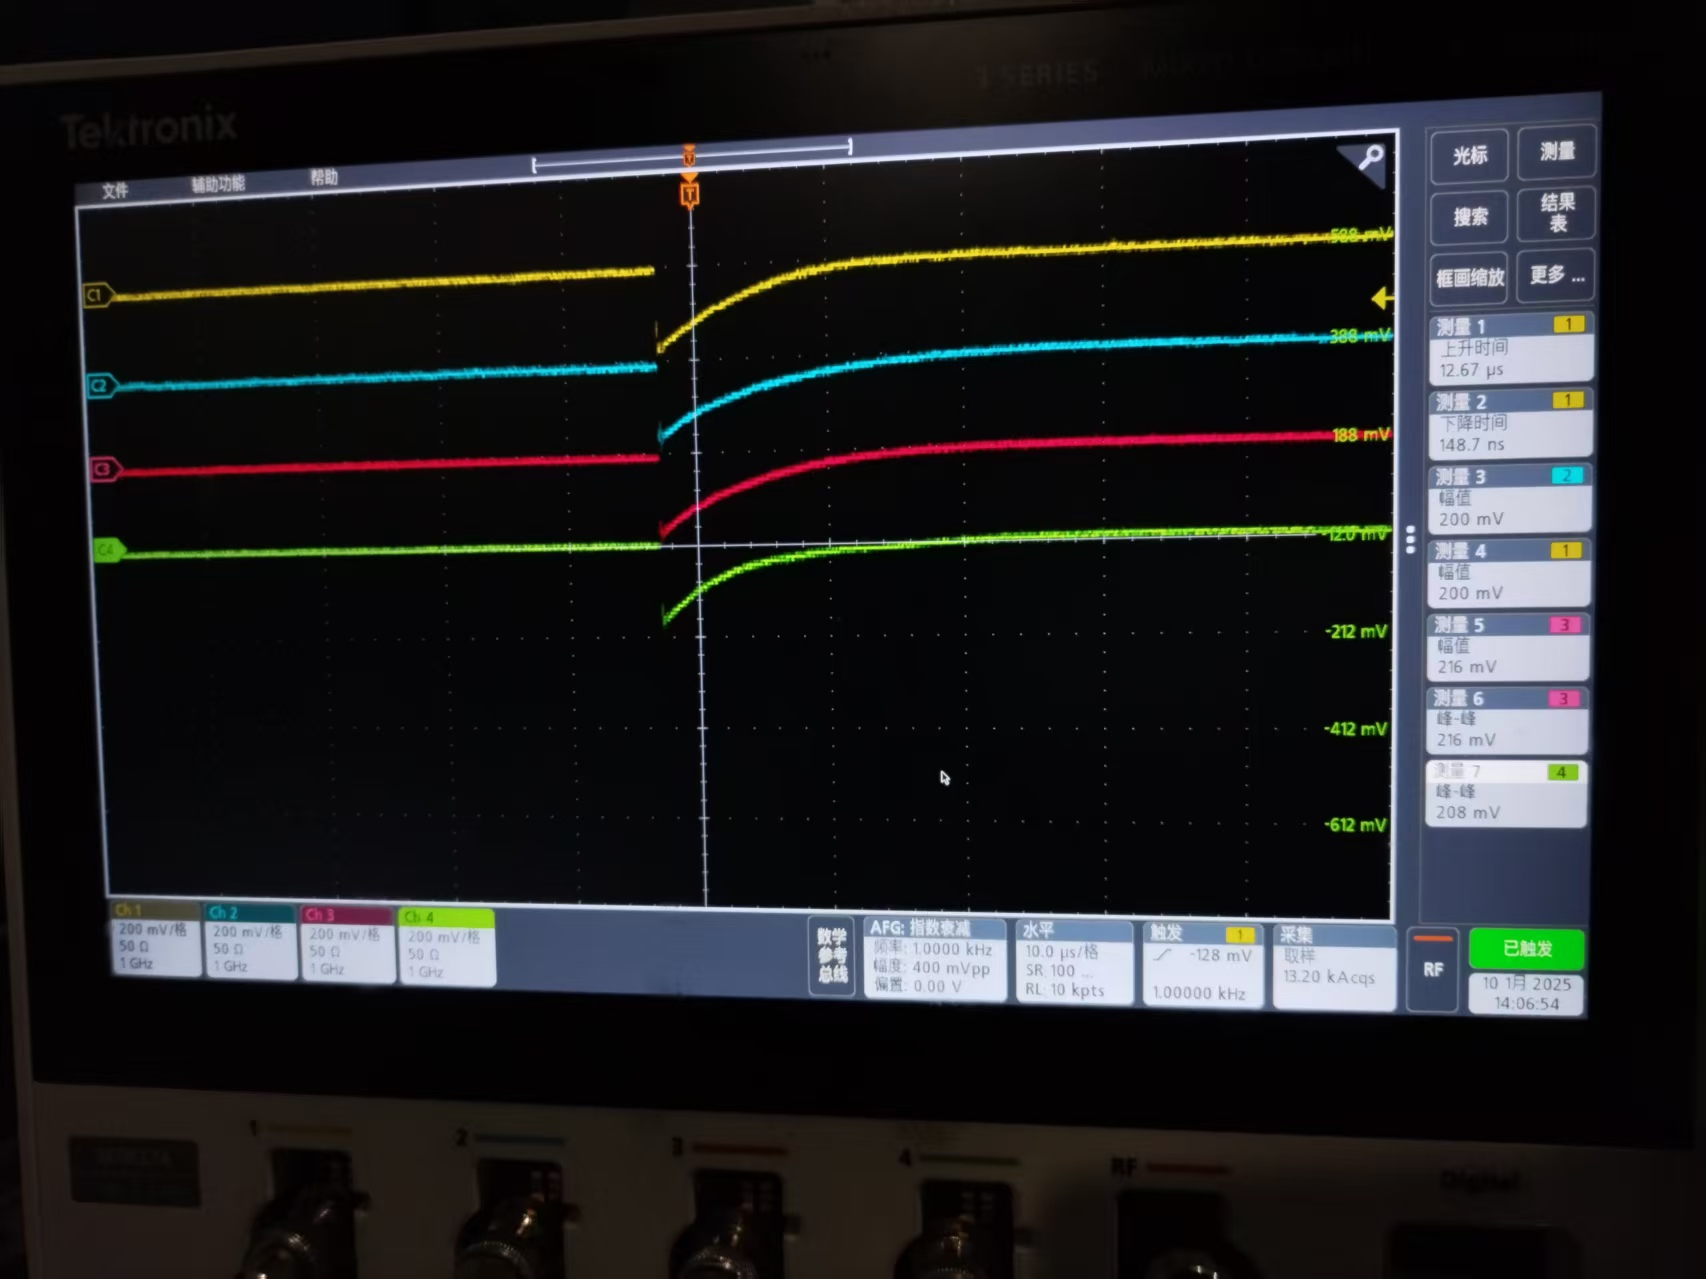
\includegraphics[width=0.6\linewidth]{images/前放Test.jpg}
\caption{前置放大器的Test信号示意图}
\label{前放Test}
\end{figure}

本次实验使用北京大学的李智焕、吴泓毅等开发的PKUVMEDAQ获取系统进行数据采集。PKUVMEDAQ获取系统可以实现对获取插件的控制，从而将获取插件上ADC得到的信号道值有组织地存储到电脑上的硬盘中。在数据处理时，需要将原始的数据文件转为root格式的数据文件，再进行事件重构等处理才能得到的位置谱。获取系统的实际运行效果如图\ref{获取}。
\begin{figure}[h]
\centering
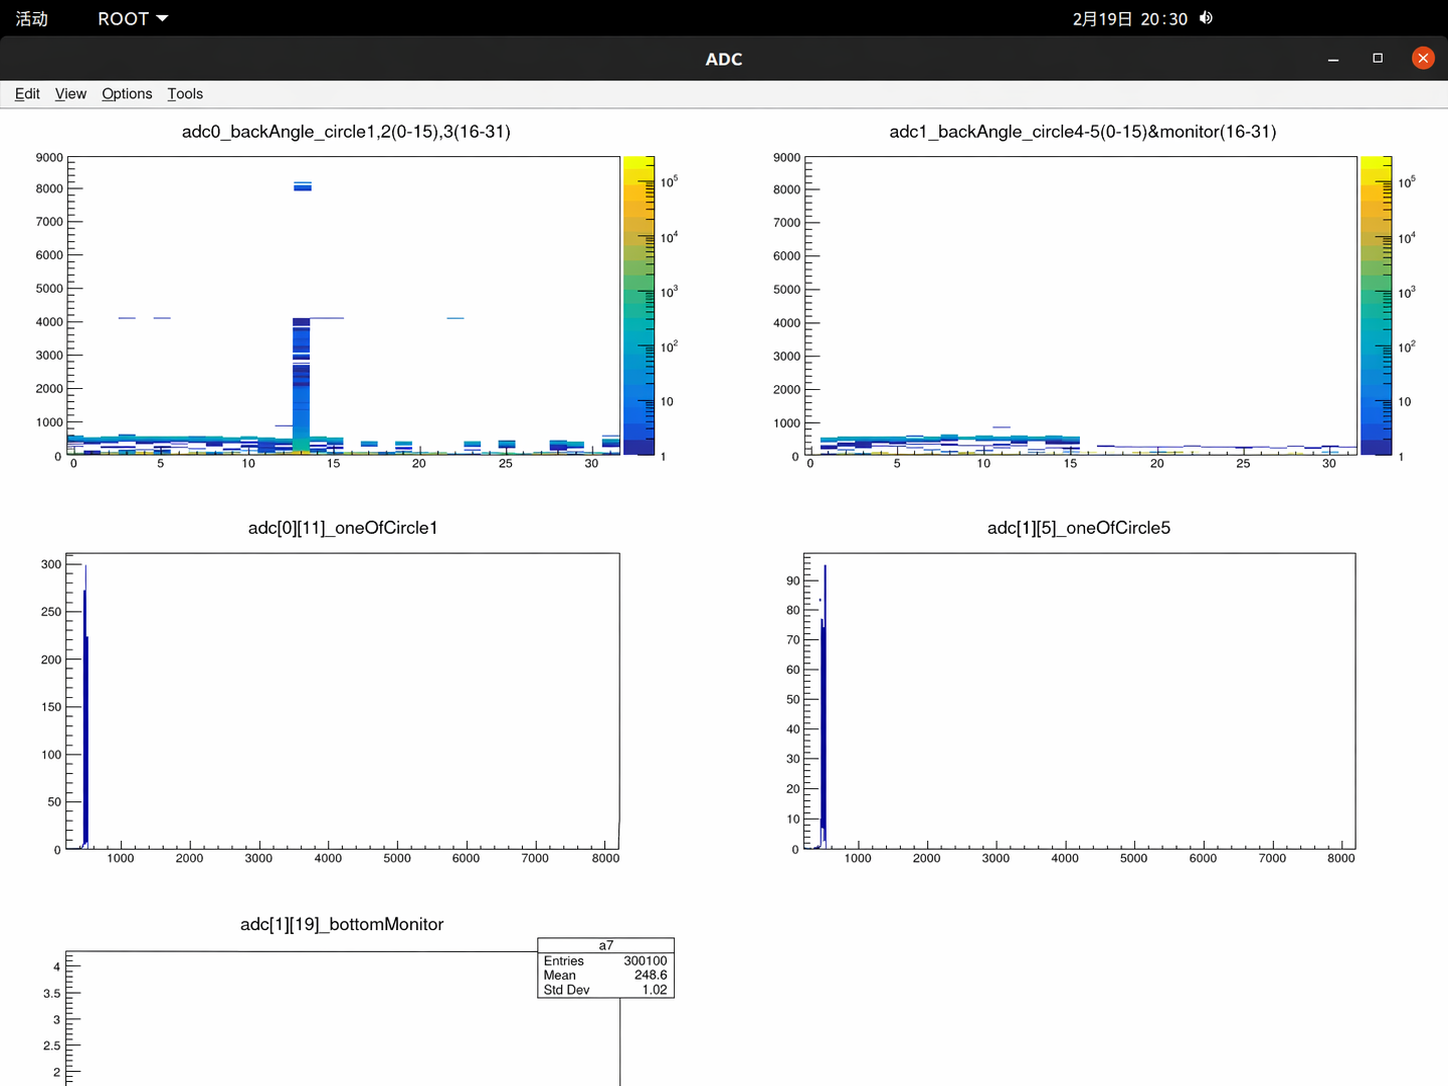
\includegraphics[width=0.6\linewidth]{images/获取.png}
\caption{获取系统的在线谱}
\label{获取}
\end{figure}


\section{实验操作}
\subsection{抽真空}
\begin{enumerate}
    \item \textbf{接线:}大靶室与外界的接线如图\ref{大靶室}所示。

    \begin{figure}[h]
        \centering
        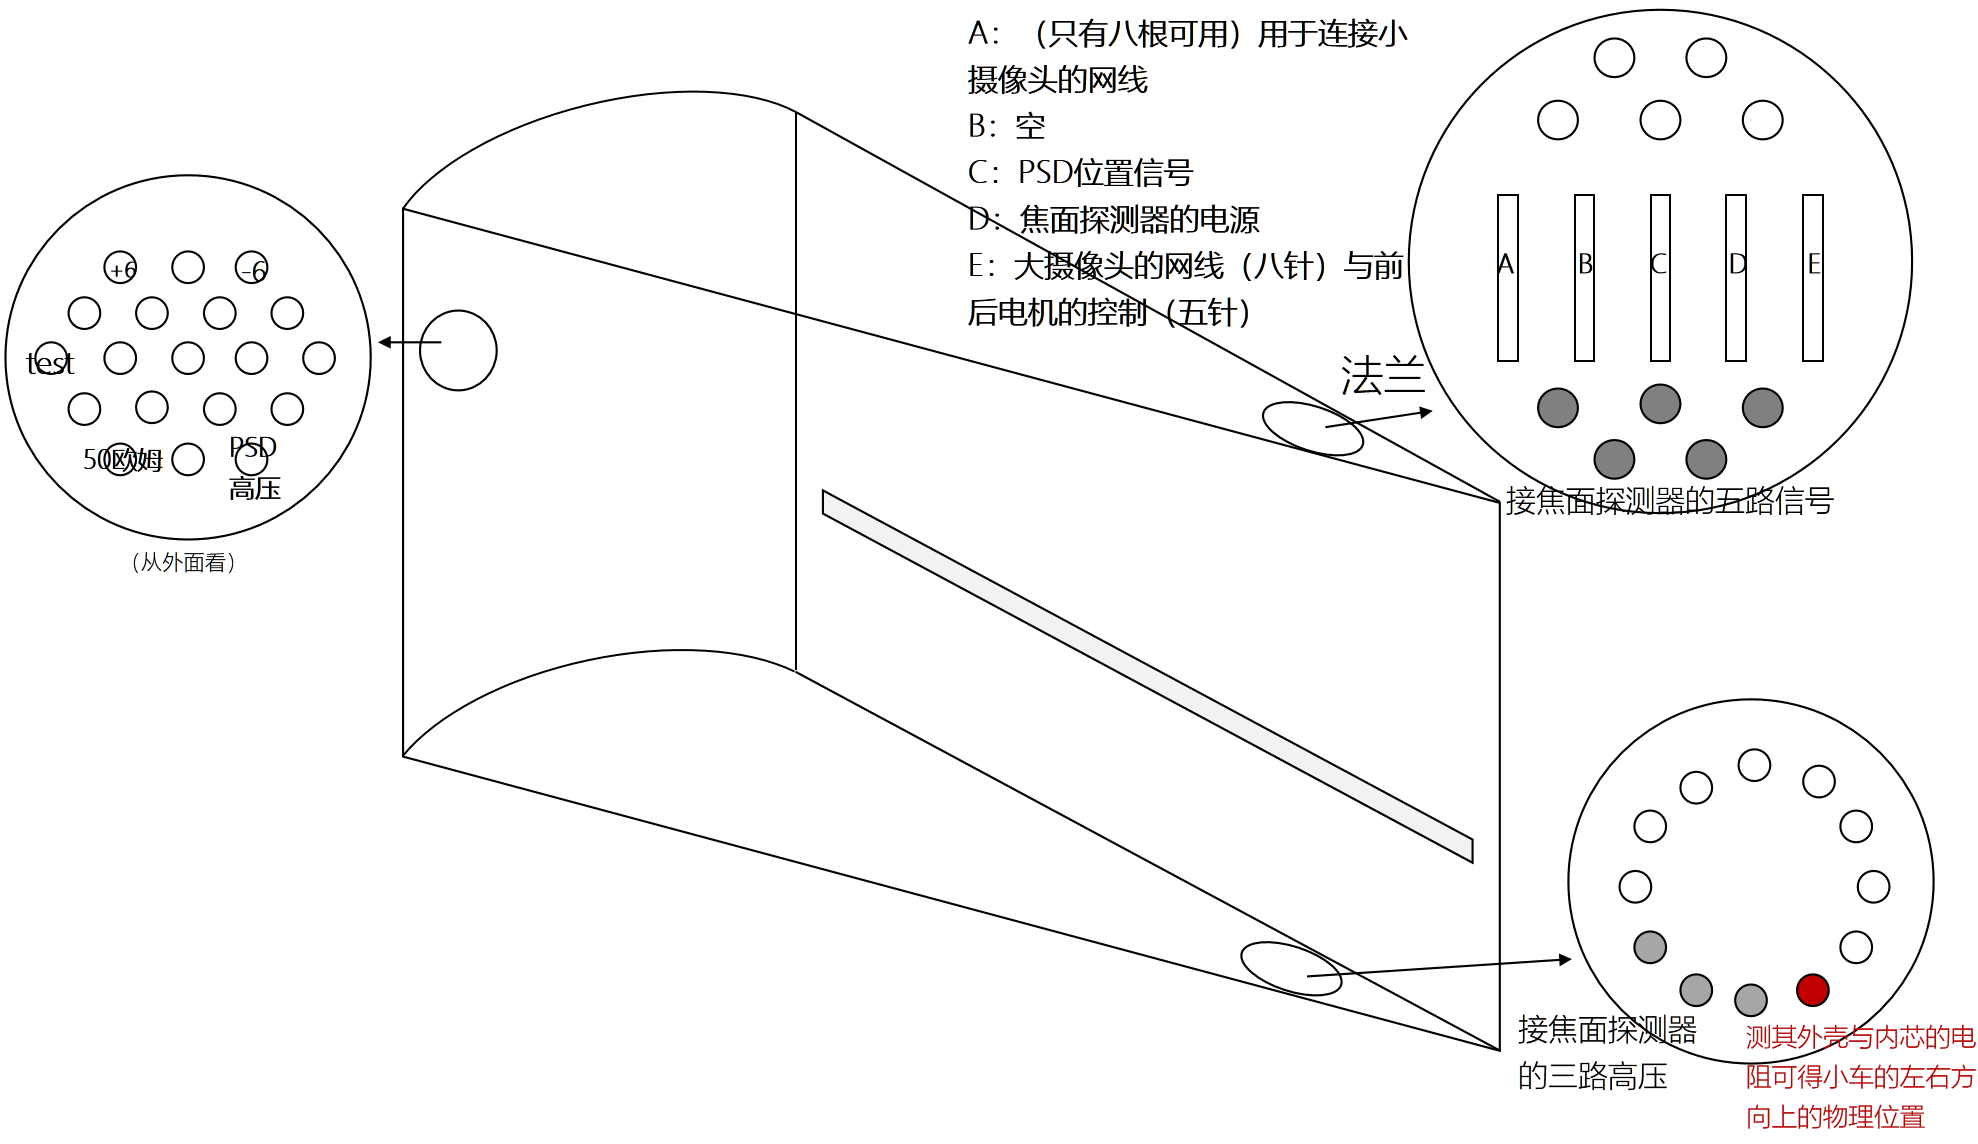
\includegraphics[width=1\linewidth]{大靶室接线 .png}
        \caption{大靶室与外界的接线}
        \label{大靶室}
    \end{figure}
    \item \textbf{关靶室盖：}
    用墙上剂量表上插的钥匙打开电箱，开关推上去，取下墙上遥控器进行操作，注意只能同时操纵一个方向。靶盖螺丝不需要拧极紧，约为手拧紧后用扳手再拧180度，隔一个空上一个螺丝即可。注意吊机使用后需放回原处，且吊机下不可放置杂物。注意靶盖不要压到电源箱电线。注意使用吊机时不要碰到天花板灯泡。

    \item \textbf{抽真空前准备：}

A.板子是否挂好；

B.PSD的安装及接线；

C.源是否装好or取下；

D.线是否可以自由移动；

E.焦探的前放与其之间的接线；

F.检查丝的电阻；

G.检查电源；

H.打开PSD及焦探的盖板；

I.看前放test信号以及噪声；

J.所有电子设备关闭；

K.放气阀关闭；

L.机械泵阀门关闭；

M.打开大靶室与焦探之间的连通。

        \begin{figure}[h]
\centering
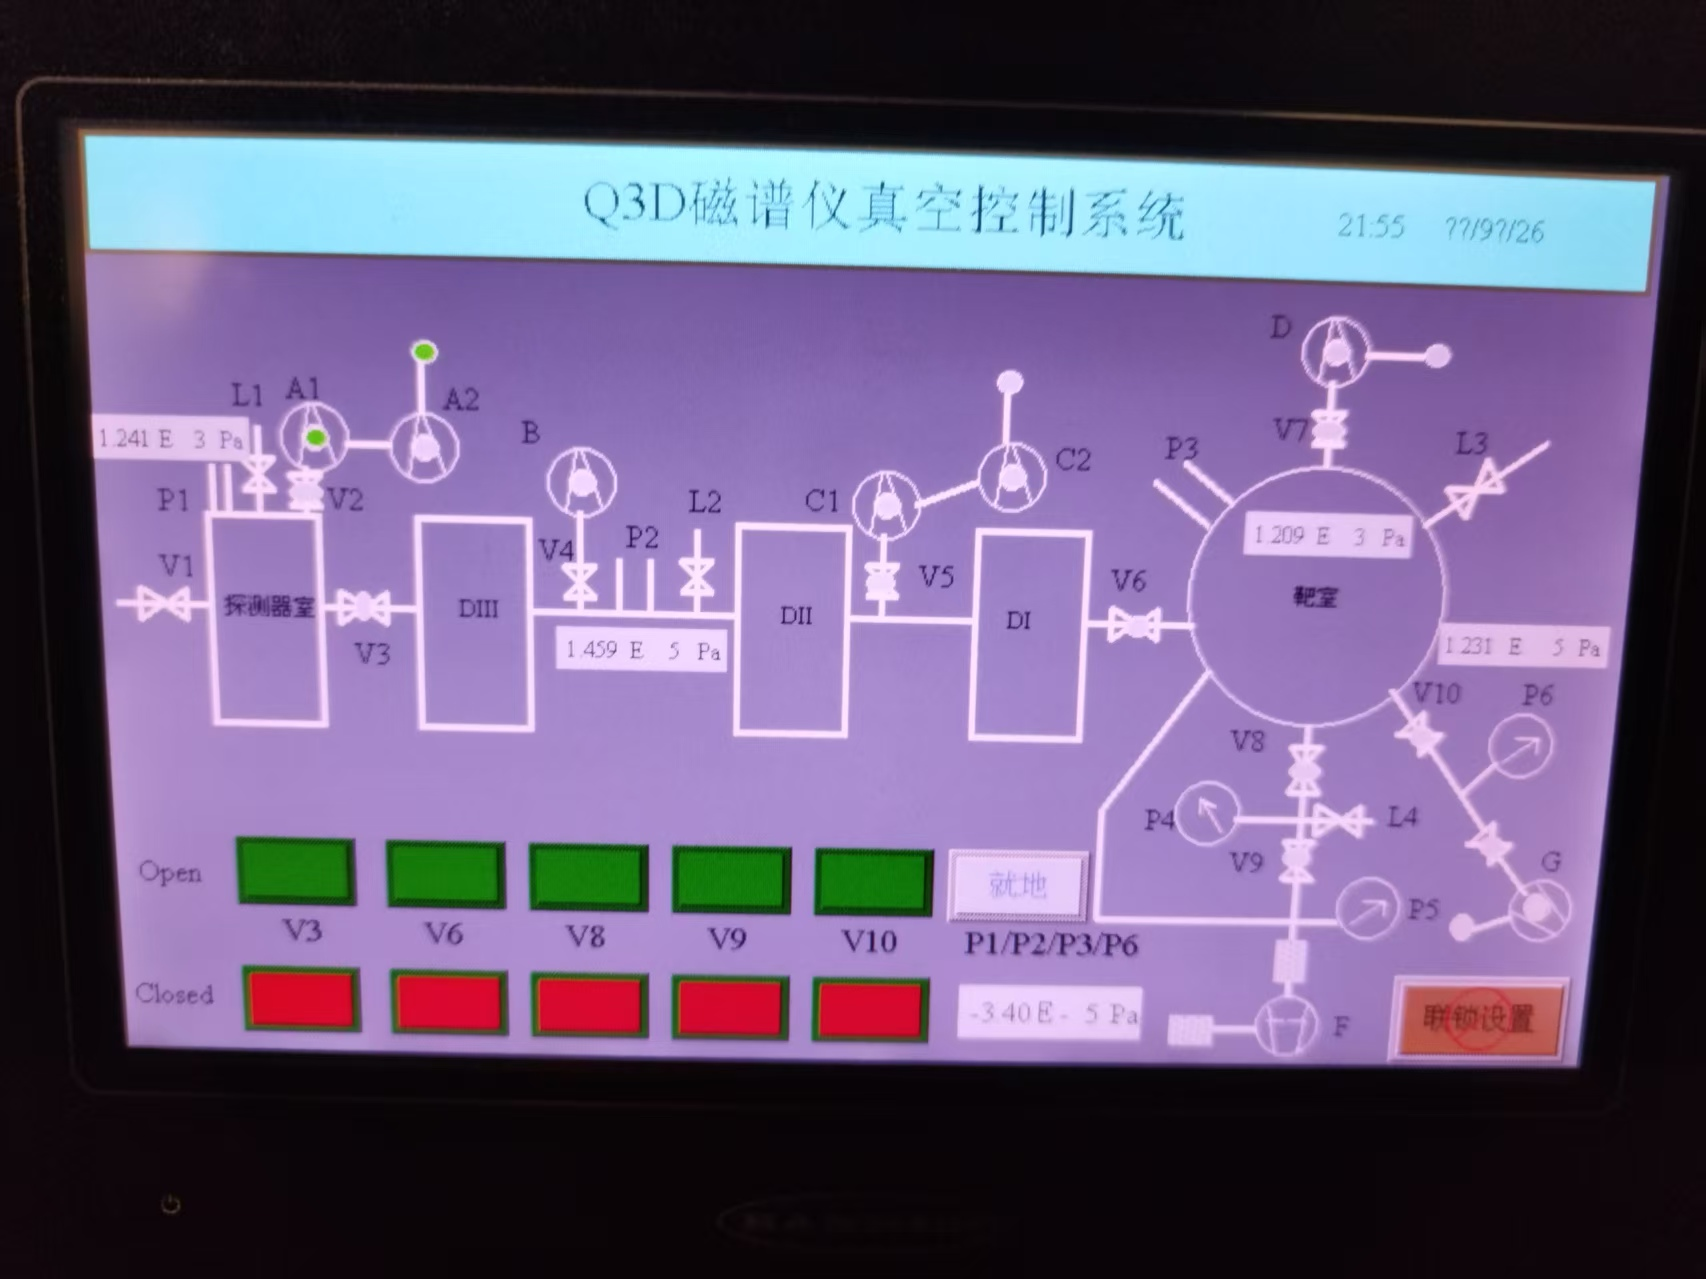
\includegraphics[width=0.95\linewidth]{images/真空控制系统.jpg}
\caption{真空控制系统示意图}
\label{真空}
\end{figure}
    \item \textbf{抽真空操作流程:}

    {\kaishu 注：操作柜的前两行气压表示数不准，以实际电离硅气压表（大靶室侧边）为准，抽2小时后约能达到e-3级别。} 
    
    A.关闭探测器高压；
    
B.打开墙上“Q3D真空”开关；

C.打开控制柜上“总电源合闸”开关，需要把抽屉抽出，同时拨动两个拨钮；

D.先打开A2机械泵，先在控制柜操作后旋转实体旋钮，控制在一秒一Torr即可（似乎实体旋钮无效）；

E.若A2已全开但下降速度仍然较慢，打开其它机械泵，其中B、D泵仅在控制柜上操作，C泵需要额外打开实体阀门，旋转使其冒白烟（这个白烟是油泵运行时泄漏出的油），待其不冒白烟后关闭（C泵位于磁铁D1和D2之间，需要绕到后面开）（D泵是抽小靶室的，大小靶室的连通靠V6控制）；

F.气压低于100 PA （0.75 Torr)时（经验为十分钟）,打开分子泵（需开水冷），通常我们会抽到1.2e-3；

G.小靶室很难抽真空抽到较低气压，通常是与大靶室连通后再继续抽，但是连通时需要注意大小靶室的气压差尽可能小。
最终，气压应该能够稳定在9e-4pa的量级，这样就足够完成实验了。
   

  \item \textbf{抽真空后对焦面探测器充气:}

  {\kaishu 注：使用CF4气体可加更高的高压而无漏流，P10气体效果略差，目前使用的是P10气体；共三个阀门，加气时旋转顺序为从探测器端到气瓶端；此处所提及的气压为焦面探测器内部气压，即机箱旁边的气压表示数。}    

A.洗气：关闭焦探与大靶室的连通（黑色拨钮90度），关闭小泵的连通（小泵用于抽气），给气瓶放气加到80 Torr(速度保持为一秒一Torr),关闭气瓶的所有出气阀门，保持焦探与大靶室的连通并极缓慢打开小泵的连通使其抽气至10 Torr，重复一次加气抽气，关闭与小泵的连接；

B.继续给气瓶放气，加到80Torr(气压表已设定为80 Torr，它会帮助调节的），在后续实验中我们发现80 Torr时第三层无信号，故将气压降为40 Torr，但是具体数值应精确计算，也许换其它气体会更好）；

% 2025/10/29更新：焦探内部气压仍然使用80 Torr.

C.加气端拧紧但留一点点（维持左边表盘0.1左右），小泵抽气端打开一点点（约为刻度5）。


  {\kaishu 注：本来打算使用丙烷气体，但是丙烷剩余量不多，故仍然使用P10.} 



    
\end{enumerate}
连通大小靶室：方法一开V6阀门（但需要在气压计显示两边压强差很小时才会被允许进行该操作），方法二（因气压计被取走修理故无法实践法一）输入联锁密码解除该设定，方法三（将小靶室边上的两根气管对调。{\kaishu 务必记得在进行后续操作时将气管换回来}


% \begin{figure}[h]
%     \centering
%     \begin{subfigure}[t]{0.48\textwidth}
%         \centering
%         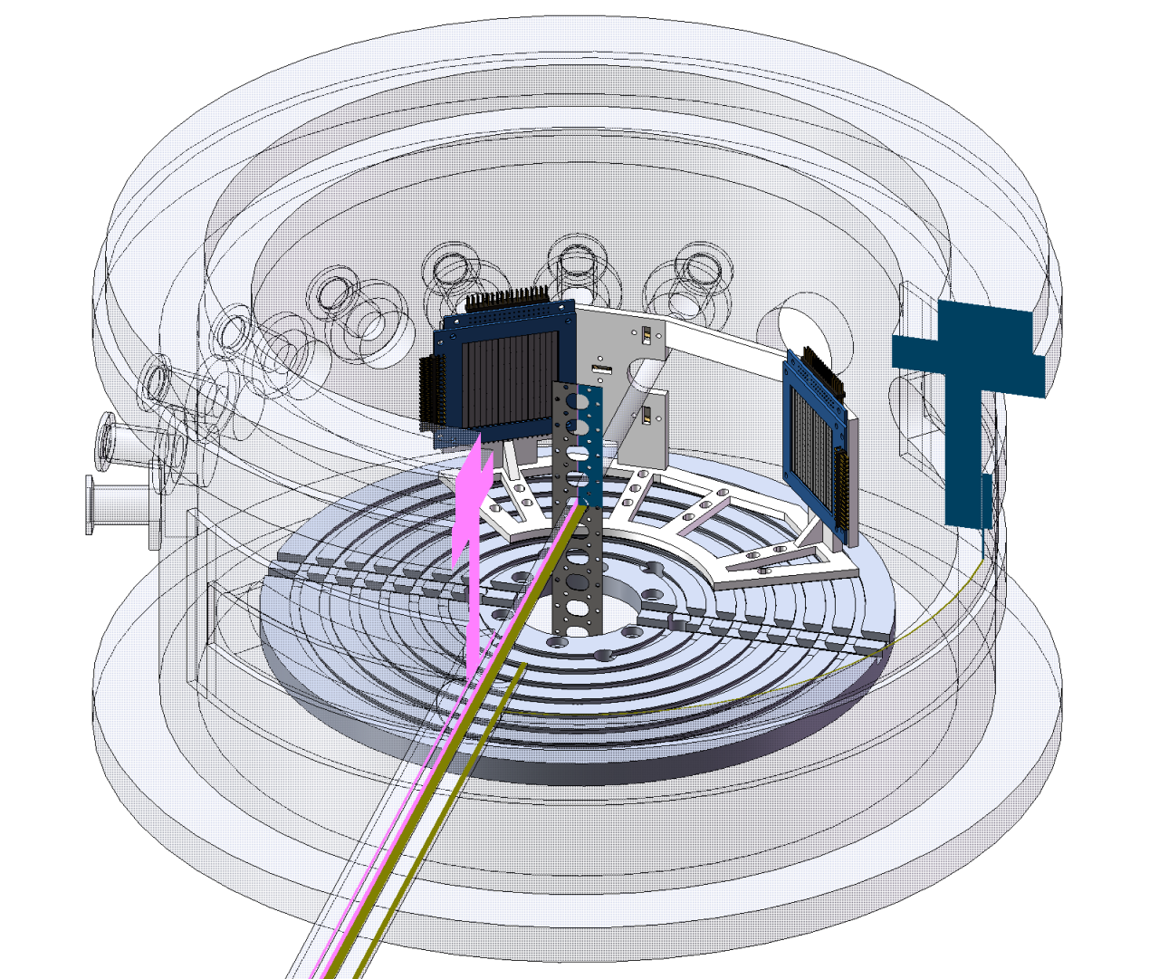
\includegraphics[width=\linewidth]{小靶室.png}
%         \caption{小靶室结构示意图}
%         \label{a}
%     \end{subfigure}
%     \hfill
%     \begin{subfigure}[t]{0.3\textwidth}
%         \centering
%         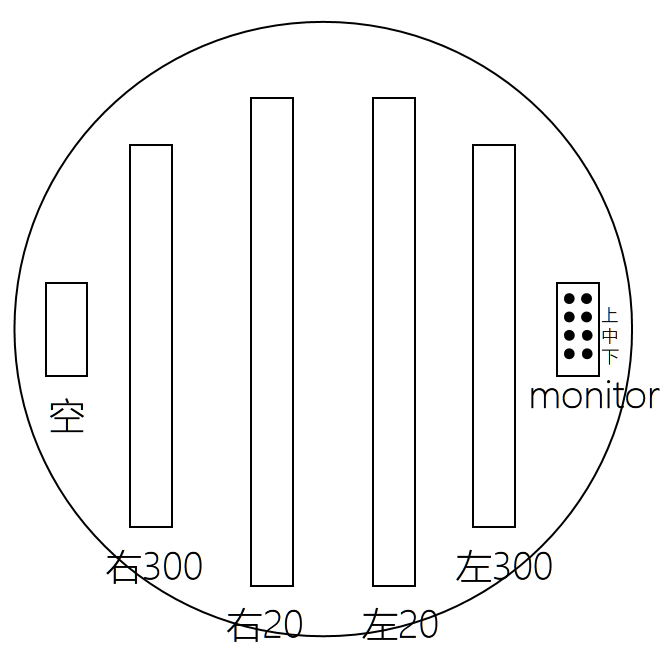
\includegraphics[width=\linewidth]{小靶室法兰.png}
%         \caption{小靶室法兰接线}
%         \label{b}
%     \end{subfigure}
%     \hfill
%     \begin{subfigure}[t]{0.2\textwidth}
%     \centering
%     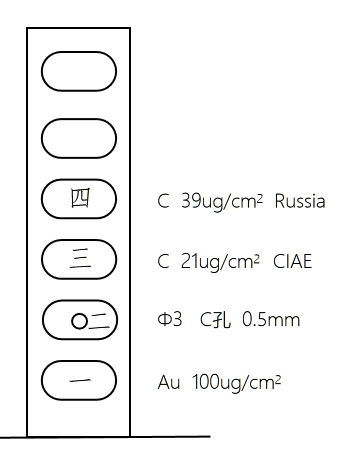
\includegraphics[width=\linewidth]{靶具体情况.png}
%     \caption{靶示意图}
%     \label{靶}
% \end{subfigure}
%  \caption{小靶室的结构及其法兰接线}
% \end{figure}


V10在实验期间需要打开，注意打开前要先打开束流管道上的四个手动阀门。注意V10不可在转动Q3D时打开。V10也可选择调节气管来控制开启or关闭。


V9是单独抽靶舱内气体的阀门，打开阀门们控制器的小门，注意门后不要碰（有220V电压），先多次点按，后持续长按。

V6和V10也可选择用控制器控制，但是需要在实验期间用扎带or胶带将按钮固定起来按住。
\subsection{Q3D磁场调节}
\begin{enumerate}

    \item 打开二厅控制电脑桌面的Q3D2文件夹里面的Q3D2文件夹，修改q3d2.inp文件（通常只需要改目标能量即可），再运行q3d2.exe文件，一直输入1回车。运行结束后，结果在Q3D2.OUT文件中，根据其目标磁场去设置电流即可。
    \item 部分电流的设定值可以通过在桌面的Q3D设场-NRGFromet.xls文件中输入对应设定值获得。
    \item BQ，BMI直接根据表格里的电流值设置最右侧机柜对应的机箱即可。
    \item M2Q,M2S,M2O,M2DE 在电脑的小电源控制软件中设置。需要保证小电源的USB盒子插入电脑。
    \item BD2 要在电脑的NetAssist软件中设置电流，具体方法参考桌面的“电源设置注意事项.txt”。随后查看其实际磁场多次调整。需要保证Q3D控制网线接入同一内网，并电脑的IP在192.168.2.x 网段。
    \item BD1 调整完BD2后，调整Trim1的电流来改变BD1的磁场值。
    \item BD1，BD2磁场查看方法：调整右侧第二个机柜的Probe（有两个Probe按钮都要调），等待面板示数稳定即为当前磁场强度。
    \item BD3 磁场查看方法：左右晃找到共振峰。比较复杂。
\end{enumerate}
\begin{figure}[h]
\centering
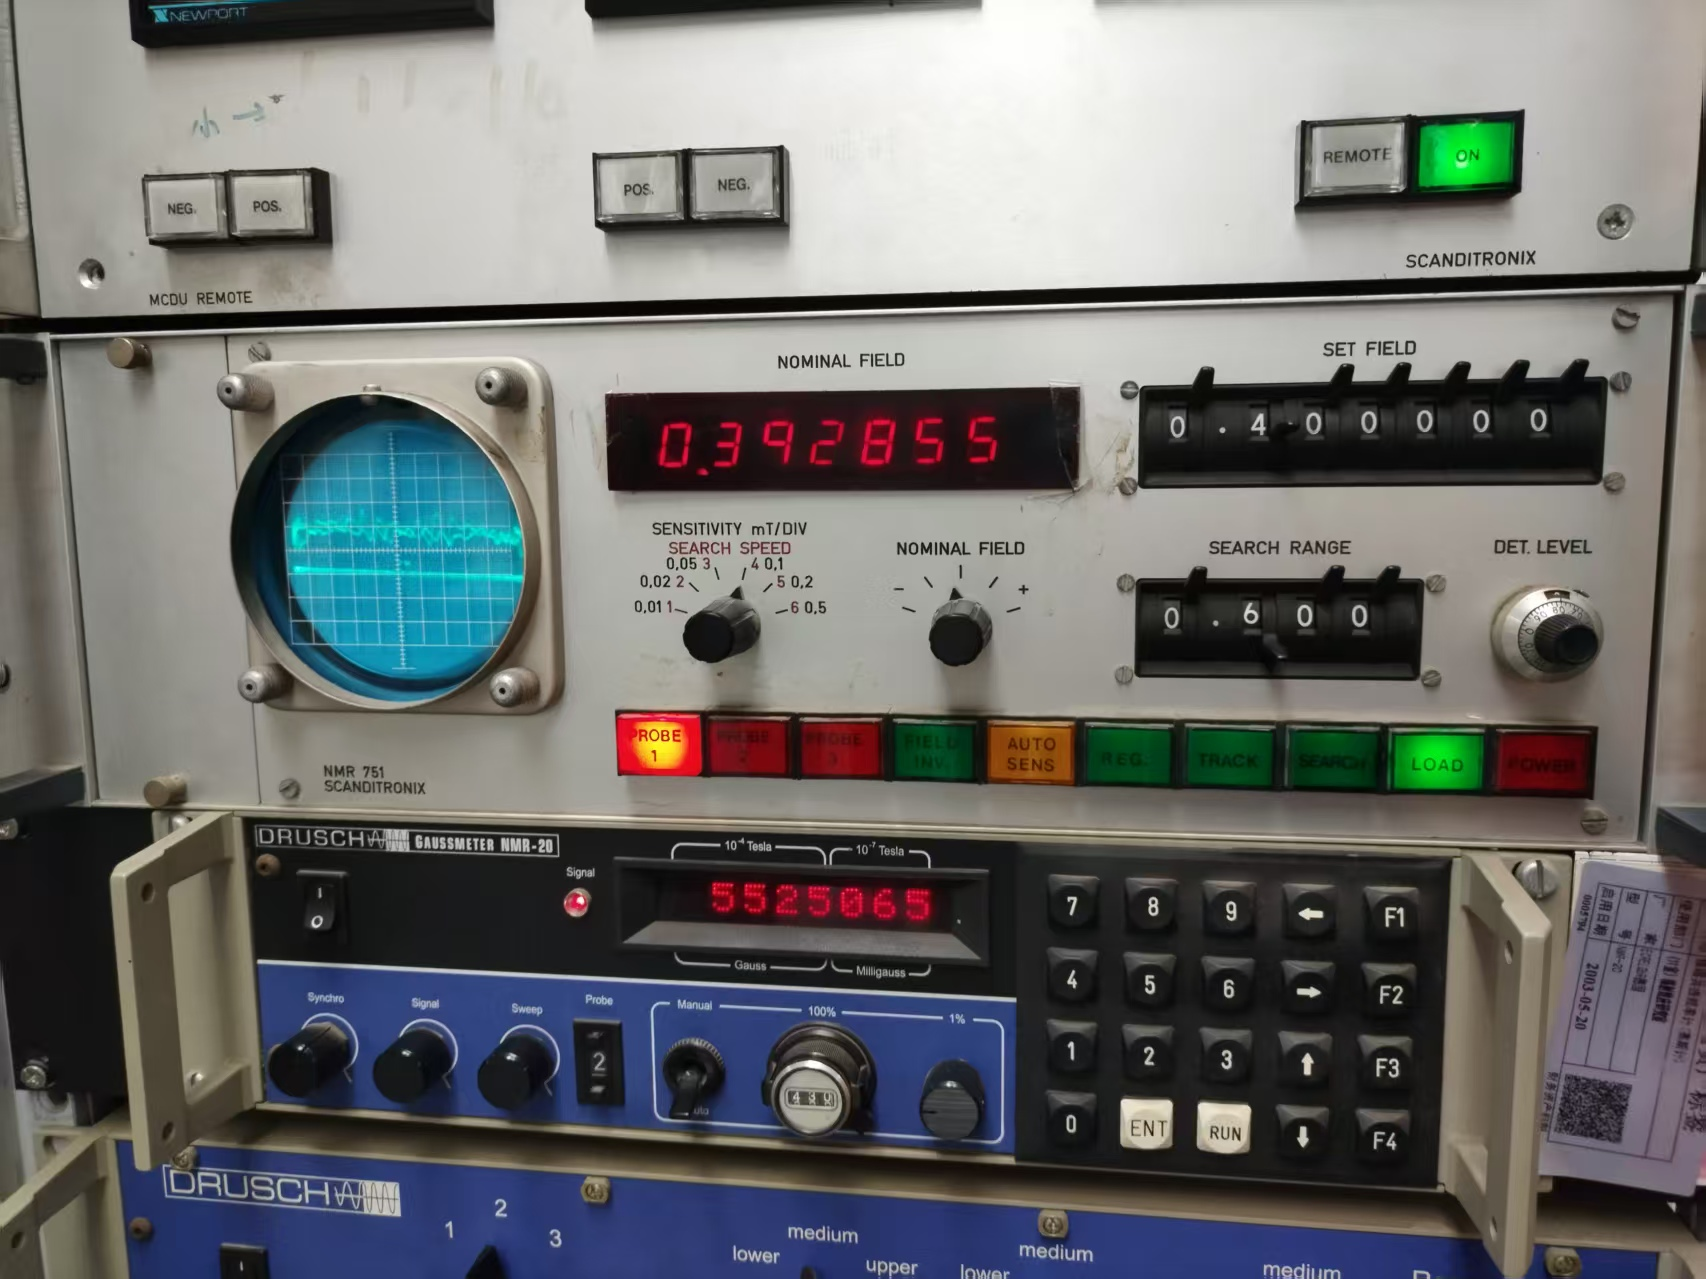
\includegraphics[width=0.95\linewidth]{images/磁场设置.jpg}
\caption{Q3D磁场设置过程图}
\label{磁场}
\end{figure}
\subsection{转动Q3D}
Q3D角度通过独立的电机控制，Q3D磁谱仪转动时将带动整个实验平台旋转，因此需同步检查电缆余量、真空连接状态及机械限位情况。实验中通常采用人工监视方式缓慢调角，以避免线缆受力或系统失稳。
要控制Q3D角度，需要将控制Q3D电机的USB盒子接入电脑。随后打开桌面的TC45运动控制系统，选择适合的com口后，即可通过+x -x来调整角度。
\subsection{靶的调节}
% 我们使用的靶包括12C靶以及197Au金靶。这些靶及其靶位在图\ref{靶}里有具体讲解。 

% 2025/10/30 20:30 在靶架的第二靶位上装了一个荧光$\Phi$3靶。

调节小靶室的靶高，可用小靶室后面的望远镜来观察调节进度。需要注意在望远镜里的视野上下是颠倒的。望远镜只有在大小靶室连通后才起效（也就是V6阀门开启后）。需要给小靶室打光。

调节靶高的方法是Q3D右边机箱上最上面一层的控制器，共有6个按钮，左边两个控制靶高，中间两个控制靶角（已失效），右边两个是开关。打开开关后，按控制靶高的左边的按钮是使得靶上升，按控制靶高的右边的按钮是使得靶下降。需要注意在望远镜里的视野上下是颠倒的。

靶高刻度（仅供参考，每次的示数会有微小变化）：一号靶位：49.4；二号靶位65.2-65.6；三号靶位:80.9；四号靶位：96.6.

实验中记录的典型靶位刻度可作为后续实验参考，但由于机械重复定位误差，每次装靶后仍需重新校准。
调节靶高也可选择使用REMOTE模式，在二厅控制箱按下REMOTE按钮后可在测量厅的右边第二个柜子最上方一格调整靶高，其示数与二厅内示数保持一致但是需要注意的是第一个数字“8”需要忽略。

调节靶角的方法是蹲下来，找一个黄铜色、直径约两厘米的小旋钮，手动旋转。
\section{实验过程}
\subsection{离线测试}
在正式供束前，进行一次完整的离线测试可以很好地对实验进行预演，提前解决实验中可能会碰到的问题。
进行离线测试有这些步骤：
（1）正确安装所有探测器及其线路，在靶的位置放置一个源（此处使用的是强$^{241}\mathrm{Am}$源）。
（2）关闭靶室盖并抽好真空。
（3）为气体探测器充入气体，给探测器加上高压。
（4）将Q3D磁谱仪转动到零度角，并启动Q3D磁谱仪电源，以强$^{241}\mathrm{Am}$源衰变的α粒子能量进行置场。
（5）查看各个通道的原始信号，调整合适的主放参数后启动获取系统。
（6）根据位置谱在获取系统中调整参数，直到获得最佳分辨。

在本次实验的离线测试中，以 5.486~MeV 的 $\alpha$ 粒子（对应 $^{241}\mathrm{Am}$ 源的主要衰变分支，分支比为 85.2\%）为中心进行置场，获得的位置谱如图 \ref{离线测试位置} 所示。根据以往使用强 $^{241}\mathrm{Am}$ 源的测试经验，谱中通常只能分辨出两个峰：分别为 5.486~MeV 的主峰，以及受到源污染后形成的 5.411~MeV 峰。也就是说，常规情况下原本的主衰变分支峰会因污染作用整体向低能方向偏移，从而表现为 5.411~MeV 的峰结构。  

然而，在本次测试得到的焦面探测器位置谱中，却观察到了三个较为明显的峰结构，其中计数最高的峰在低能侧似乎还带有额外的肩峰或次级结构。这表明此次测试的能量分辨能力较以往结果有所提高，使得原先难以区分的不同衰变分支得以显现。结合 $^{241}\mathrm{Am}$ 的衰变数据分析，可判断谱中第二高能位置的峰应对应于 5.443~MeV 的次要衰变分支（分支比为 12.8\%）；而最大峰低能侧所附带的结构，则应为该 5.443~MeV 分支在源污染影响下向低能移动后形成的对应峰。  

同时考虑第一、三层的位置谱，可以还原出粒子在焦面探测器内的二维飞行轨迹如图\ref{离线测试径迹}。5.443~MeV的粒子在两层的位置被圈出，可以看到在第一层能量被识别该5.443~MeV的粒子到了第三层仍然在同样的位置，径迹也与其它大部分的粒子径迹平行，这为识别结果提高了可靠性。

根据峰对应的能量以及拟合得到的高斯峰参数可以计算得到最高能峰的能量展宽约为0.27\%。这一测试说明，在考虑了源本身的污染以及能量展宽的情况下，最终的分辨仍然要比0.27\%更好。尽管这与理论的0.01\%级的探测能力还有差距，但也远远好于以往其它的探测体系了。

焦面探测器及其电子学系统在离线测试条件下表现出了较好的位置分辨能力和峰结构分离能力，为后续在线实验中不同反应道峰位的识别与计数分析提供了有利条件。

\begin{figure}[h]
\centering
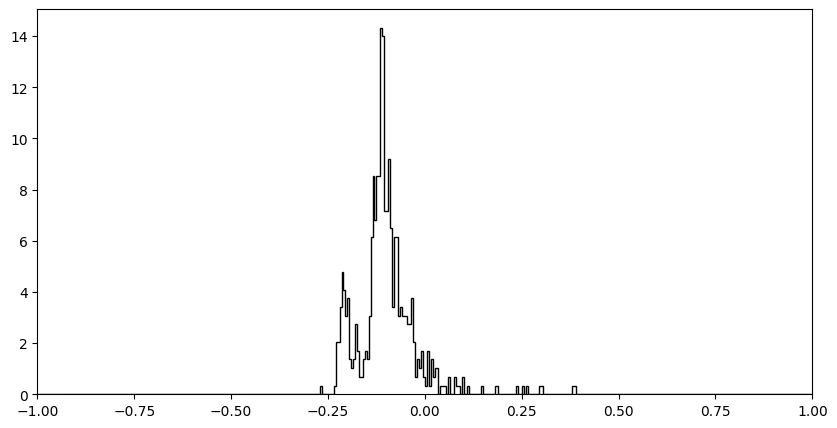
\includegraphics[width=0.8\linewidth]{images/离线测试位置.jpg}
\caption{离线测试位置谱}
\small 负方向为高能端，正方向为低能端。
\label{离线测试位置}
\end{figure}
\begin{figure}[h]
\centering
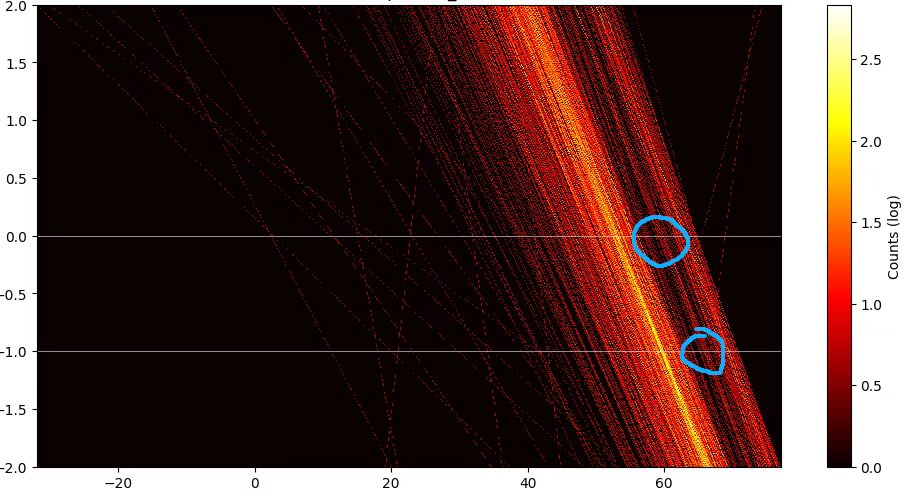
\includegraphics[width=0.8\linewidth]{images/离线测试径迹.jpg}
\caption{离线测试径迹谱，蓝圈示意5.443MeV的α粒子在第一、三层的位置}
\label{离线测试径迹}
\end{figure}
\subsection{束流调节}
正式上实验后的第一步就是进行束流的调节。靶架上除了实验目标的$^{152}\mathrm{Sm}$靶还放置了一个荧光靶，这样只需观察到荧光靶上的亮斑向中心的φ3孔移动随后逐渐消失，就可以知道束流调好了。束流接近调好的状态如图\ref{调束}。
\begin{figure}[h]
\centering
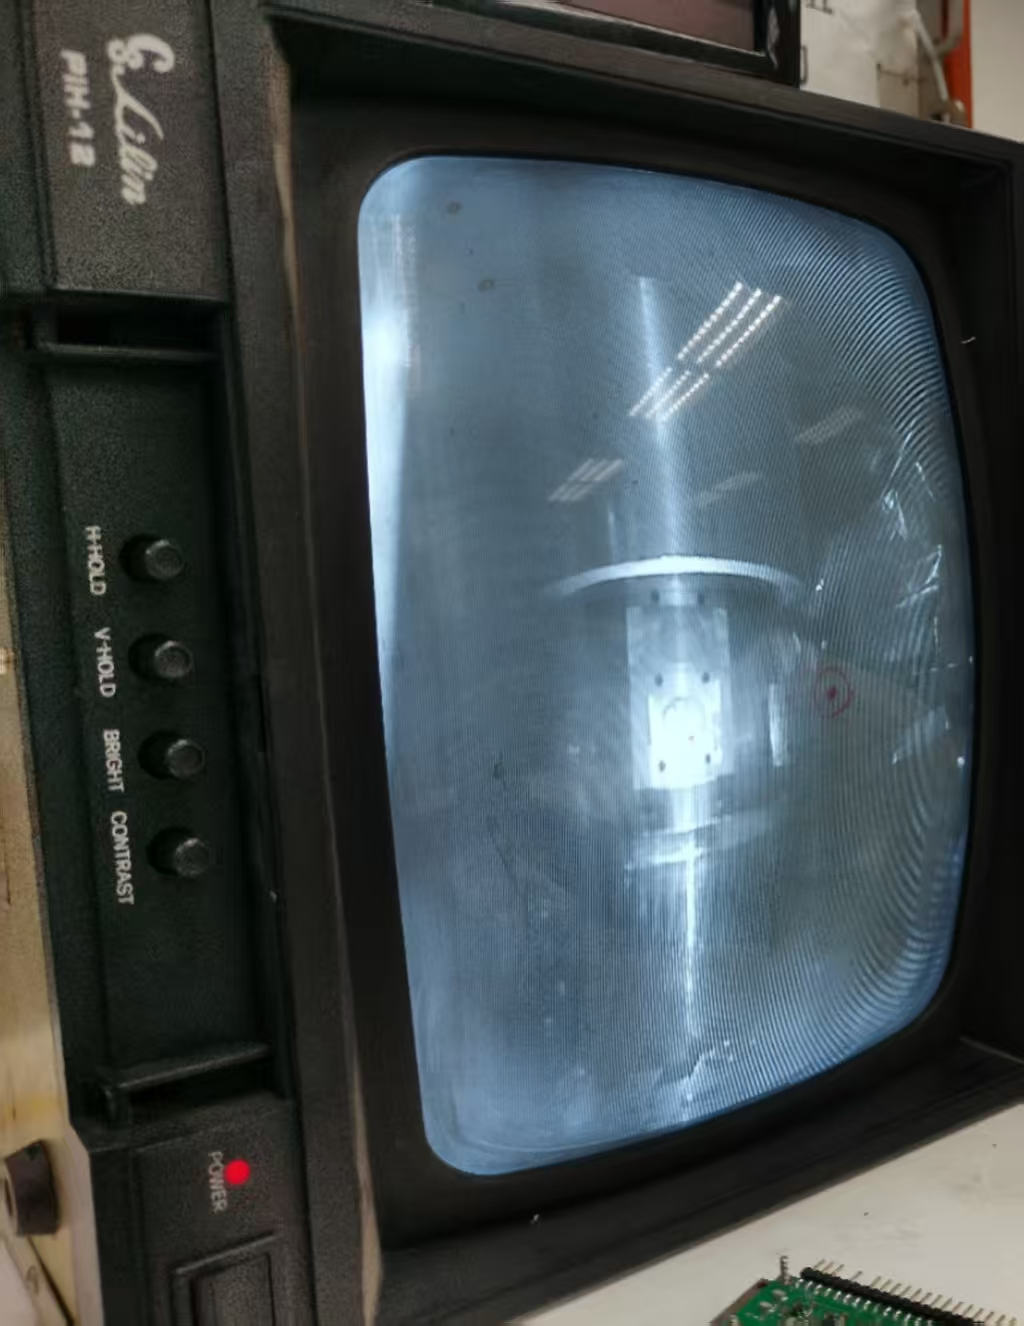
\includegraphics[width=0.6\linewidth]{images/调束.jpg}
\caption{调束过程图}
\label{调束}
\end{figure}
\subsection{焦面探测器位置调整}
由于当时大靶室内的电机被卸下，想要对焦面探测器进行位置调整就非常困难，需要打开大靶室再人工调整探测器的前后位置。并且实验中发现原先大靶室吊挂滑轨的调整范围有限，不得不将焦面探测器直接放在铁架上来寻找最佳焦面位置，整个过程非常艰难。最后调整好的焦面探测器位置如图\ref{焦面探测器位置图}
\begin{figure}[h]
\centering
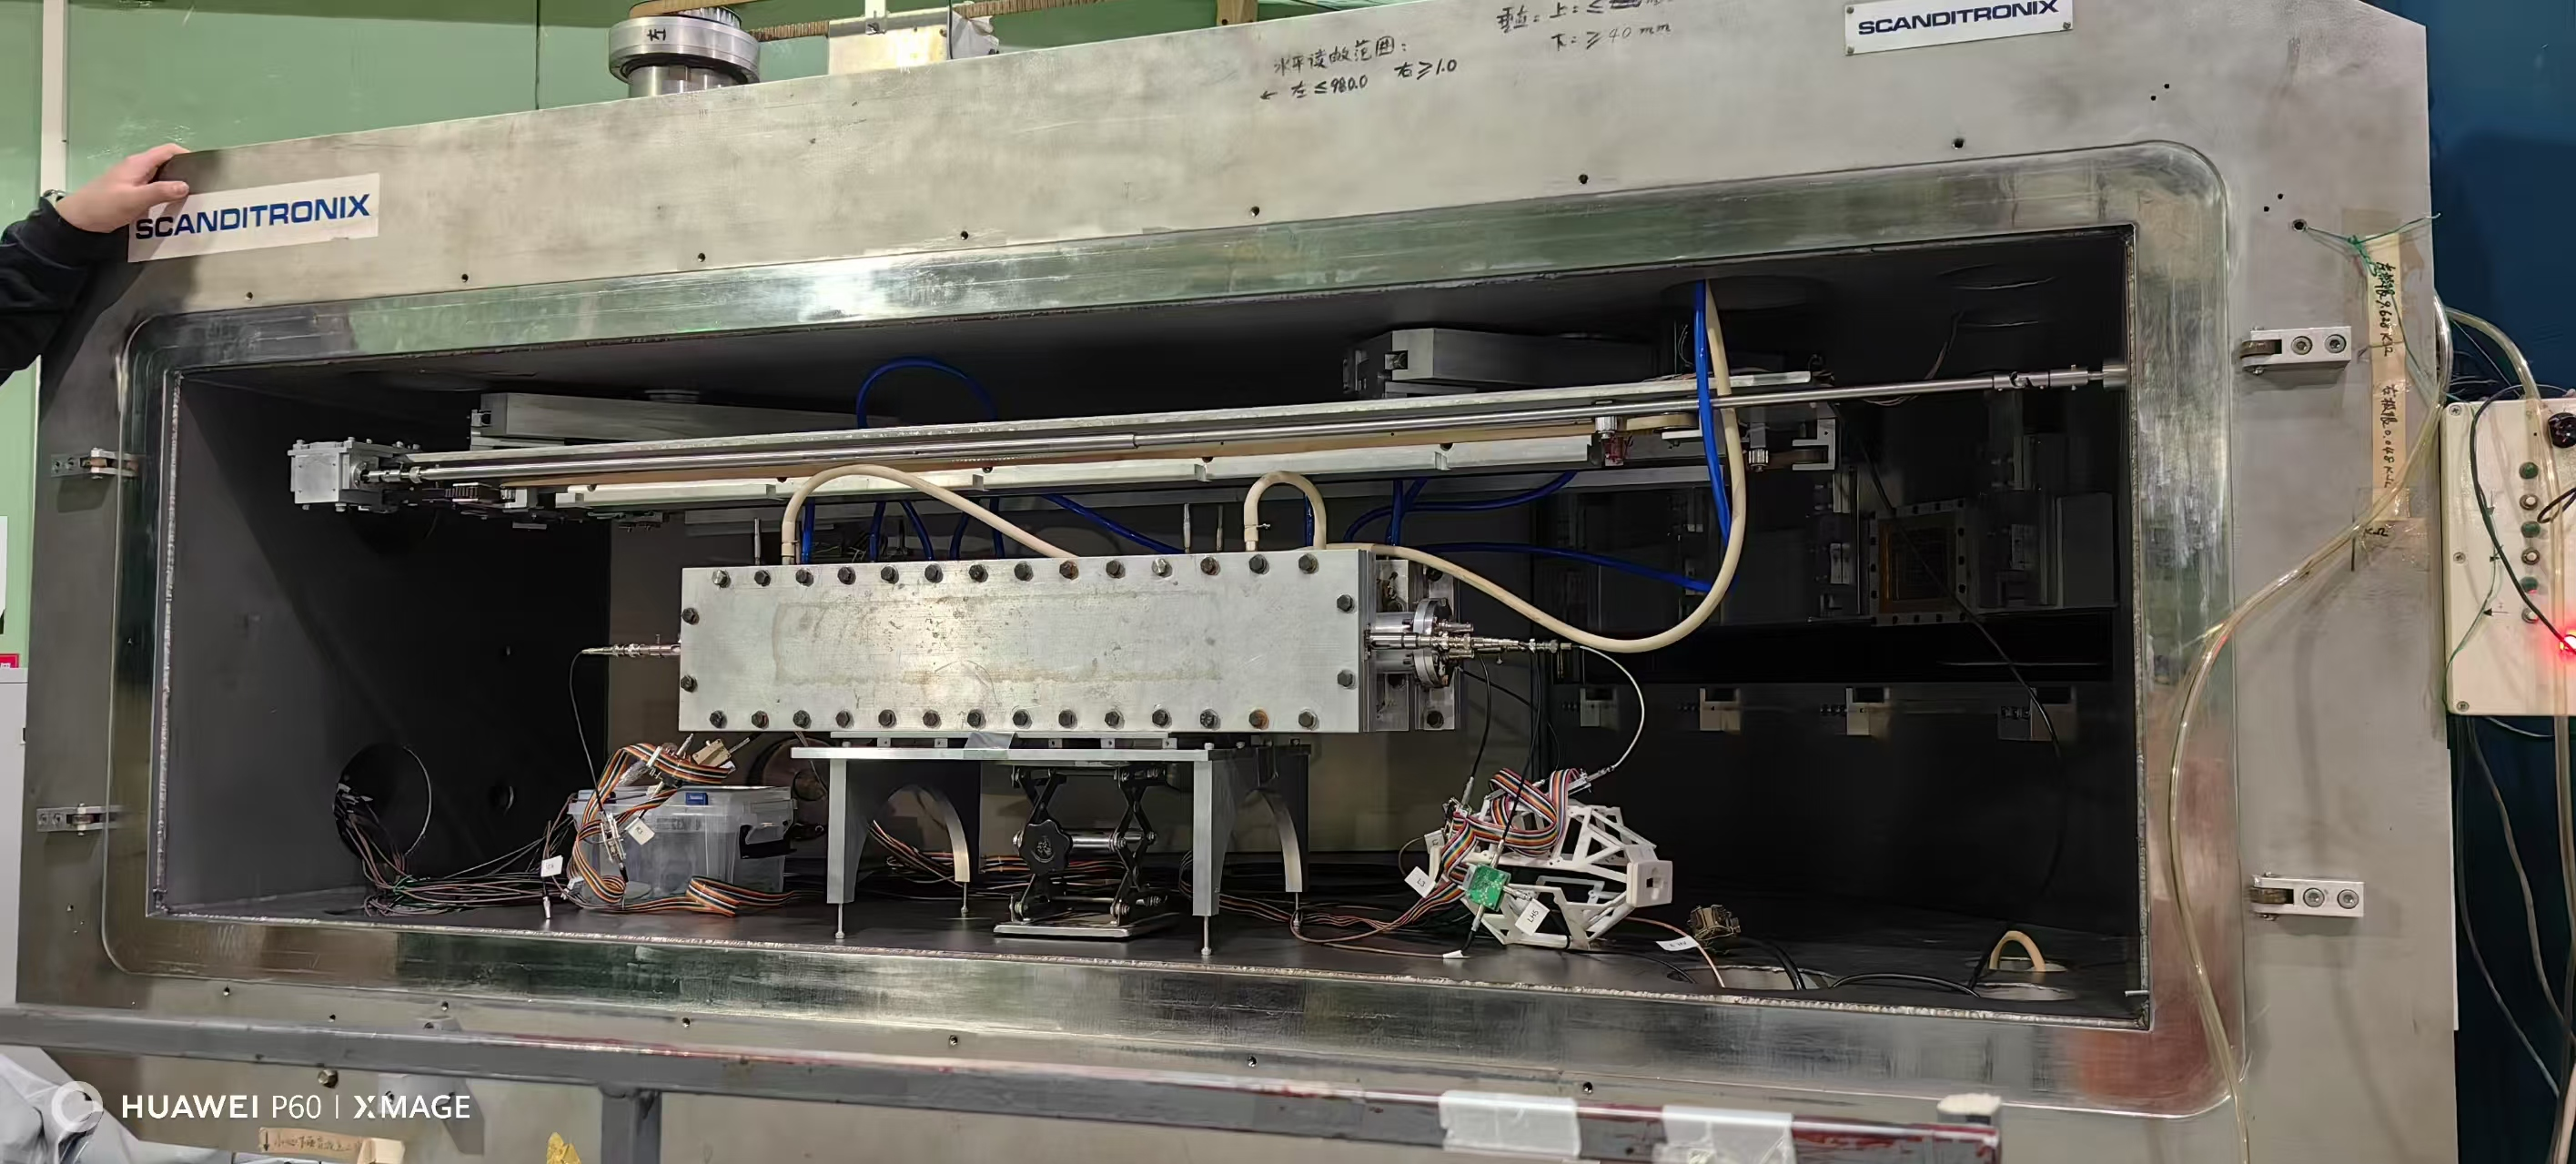
\includegraphics[width=0.8\linewidth]{images/焦面探测器位置图.jpg}
\caption{焦面探测器位置图}
\label{焦面探测器位置图}
\end{figure}

\subsection{动量刻度}
动量刻度是实验中非常重要的一环。由于实验中是通过焦面探测器的位置探测器两端的信号进行电荷相除法得到的范围从-1到1的一个相对的位置，因此需建立焦面相对位置与粒子动量偏差之间的对应关系。
考虑到实验本身就需要逐步转动Q3D磁谱仪以实现各个角度的测量，而各个角度下出射粒子的能量是可以简单又确定地进行计算，所以可以保持Q3D磁场不变，并不断改变Q3D的角度，随后就可以根据不同角度下的弹散峰的位置以及动量差来找到两者的映射关系。
图\ref{动量刻度图}中，横坐标为弹散峰的相对位置，纵坐标为运动学计算的各个角度下出射粒子的动量差，两条线以及线上的点分别为两个置场下不同角度的相对位置与动量差。由图可知，两条线的线性都很好，并且斜率都在-0.0351附近，那么这就是位置与动量差的刻度系数了。

\begin{figure}[h]
\centering
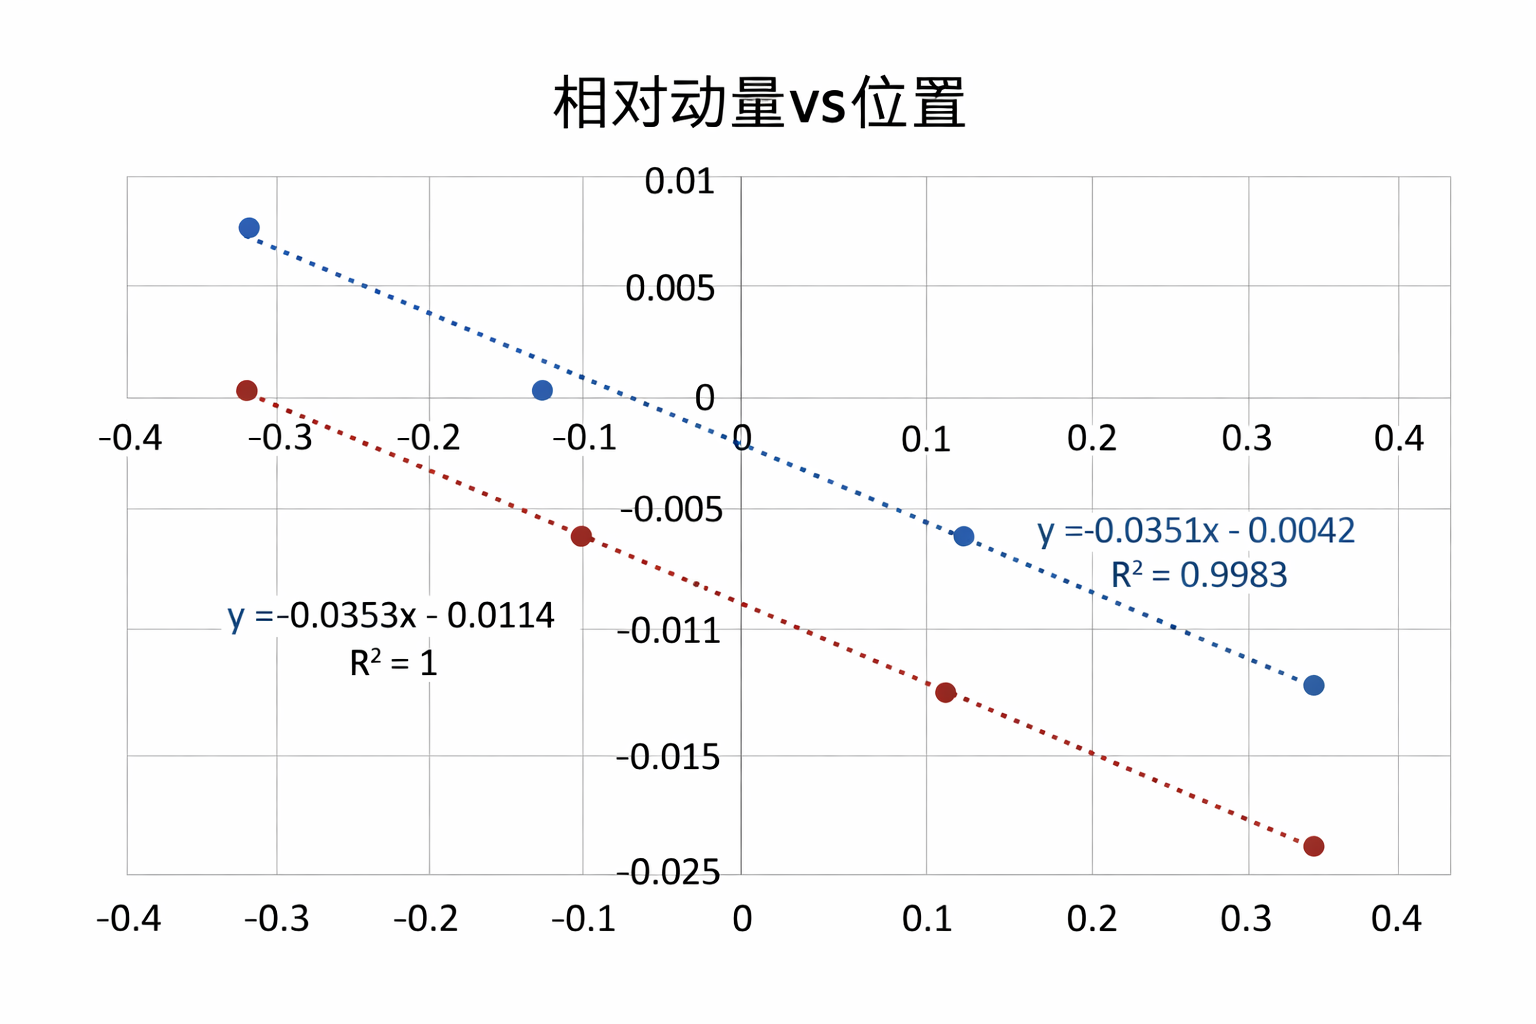
\includegraphics[width=0.8\linewidth]{images/刻度.png}
\caption{动量刻度图}
\label{动量刻度图}
\end{figure}

\subsection{立体角刻度}

立体角刻度的理论依据是，当能量远低于库仑势垒时，角分布将会趋近于一条在1附近的直线，也就是几乎只发生卢瑟福散射。在实验中，我们选择52MeV能点，换用$^{197}\mathrm{Au}$靶进行立体角刻度。
假定第 \( m \) 个PIN监视器所处的方位角为 \( \theta_{M_0,m} \)，其相对靶点的立体角为 \( \Omega_{M_0,m} \)，  
第 \( i \) 个探测器所处的方位角为 \( \theta_i \)，相对靶点的立体角为 \( \Omega_i \)。流强为 \( I \) 的 \( ^18O \) 束流入射  
到单位面积上的核数为 \( N_s \) 的 \( ^{197}Au \) 靶上，单位时间内散射到监视器的 \( ^18O \) 粒子数为  
\( N_{M_0,m} \)，散射进入第 \( i \) 个探测器的 \( ^18O \) 粒子数为 \( N_i \)。根据截面计算公式，\( ^18O + ^{197}Au \) 体系在角度 \( \theta_{M_0,m} \) 和 \( \theta_i \) 的弹性散射微分截面为：

\begin{equation}
d\sigma_{El}(\theta_{M_0,m}) = \frac{dN_{M_0,m}}{IN_s d\Omega_{M_0,m}} 
\end{equation}

\begin{equation}
d\sigma_{El}(\theta_i) = \frac{dN_i}{IN_s d\Omega_i}
\end{equation}

两式相比得到：

\begin{equation}
\frac{d\Omega_i}{d\Omega_{M_0,m}} = \frac{dN_i}{dN_{M_0,m}} \cdot \frac{d\sigma_{El}(\theta_{M_0,m})}{d\sigma_{El}(\theta_i)}
\end{equation}

另根据 Rutherford 散射截面公式：

\begin{equation}
d\sigma_R(\theta_c) = \frac{a^2}{4} \cdot \frac{1}{\sin^4(\theta_c / 2)}
\end{equation}

（其中 \( a \) 为对心碰撞时最趋近距离的一半，\( \theta_c \) 为质心系角度），可知，

\begin{equation}
\frac{d\Omega_i}{d\Omega_{M_0,m}} = \frac{dN_i}{dN_{M_0,m}} \cdot \frac{\sin^4(\theta_{C,i}/2)}{\sin^4(\theta_{C,M_0,m}/2)}
\label{eq:4.5}
\end{equation}

则根据 \eqref{eq:4.5} 式即可求出各探测器相对于监视器的立体角。实际应用中，将各探测器相对两个监视器的立体角取平均，以平均值作为探测器的相对立体角。
\subsection{测量}
实验从2025年1月18日开始，1月22日结束。前两天的主要实验内容就是根据位置谱通过多种手段调整分辨，包括调整焦面位置、调整束流、调整气压以及高压等等。后面三天进入流程化的测量。在正式的测量中，分别调节束流能量分别为 72、68、64、60、56 和52~MeV，并将Q3D磁谱仪在30-140°之间以4-5°的间隔进行转动，得到了该角度范围内的弹性散射角分布数据。前角包含信息量较少，角度间隔可以选大一些；背角或者能量较高时角分布变化更显著，角度间隔可以选小一些，当然也要适当考虑截面的因素。随着角度增加，谱中的位置峰将会逐渐向低能端移动，因此需要每次转动Q3D磁谱仪后都要检查焦面探测器的位置谱，避免束流超出探测器的窗口范围。每次束流即将超出窗口范围前，都应该重新设置磁场，并且新的磁场中心要按照比目前角度更大的情形来设置，这样下一轮的位置峰就会出现在偏高能端的位置，这样可以减少调整磁场的次数。
本次实验共完成316轮次数据获取，覆盖6个束流能点及$30^\circ\!-\!140^\circ$角区，为后续角分布提取与光学模型分析提供了充足的数据基础。由于部分大角度位置截面较低，测量时间明显长于前角区域，因此整体实验时间主要消耗在后角低计数区数据积累上。

